\documentclass[twoside]{book}

% Packages required by doxygen
\usepackage{fixltx2e}
\usepackage{calc}
\usepackage{doxygen}
\usepackage[export]{adjustbox} % also loads graphicx
\usepackage{graphicx}
\usepackage[utf8]{inputenc}
\usepackage{makeidx}
\usepackage{multicol}
\usepackage{multirow}
\PassOptionsToPackage{warn}{textcomp}
\usepackage{textcomp}
\usepackage[nointegrals]{wasysym}
\usepackage[table]{xcolor}

% Font selection
\usepackage[T1]{fontenc}
\usepackage[scaled=.90]{helvet}
\usepackage{courier}
\usepackage{amssymb}
\usepackage{sectsty}
\renewcommand{\familydefault}{\sfdefault}
\allsectionsfont{%
  \fontseries{bc}\selectfont%
  \color{darkgray}%
}
\renewcommand{\DoxyLabelFont}{%
  \fontseries{bc}\selectfont%
  \color{darkgray}%
}
\newcommand{\+}{\discretionary{\mbox{\scriptsize$\hookleftarrow$}}{}{}}

% Page & text layout
\usepackage{geometry}
\geometry{%
  a4paper,%
  top=2.5cm,%
  bottom=2.5cm,%
  left=2.5cm,%
  right=2.5cm%
}
\tolerance=750
\hfuzz=15pt
\hbadness=750
\setlength{\emergencystretch}{15pt}
\setlength{\parindent}{0cm}
\setlength{\parskip}{3ex plus 2ex minus 2ex}
\makeatletter
\renewcommand{\paragraph}{%
  \@startsection{paragraph}{4}{0ex}{-1.0ex}{1.0ex}{%
    \normalfont\normalsize\bfseries\SS@parafont%
  }%
}
\renewcommand{\subparagraph}{%
  \@startsection{subparagraph}{5}{0ex}{-1.0ex}{1.0ex}{%
    \normalfont\normalsize\bfseries\SS@subparafont%
  }%
}
\makeatother

% Headers & footers
\usepackage{fancyhdr}
\pagestyle{fancyplain}
\fancyhead[LE]{\fancyplain{}{\bfseries\thepage}}
\fancyhead[CE]{\fancyplain{}{}}
\fancyhead[RE]{\fancyplain{}{\bfseries\leftmark}}
\fancyhead[LO]{\fancyplain{}{\bfseries\rightmark}}
\fancyhead[CO]{\fancyplain{}{}}
\fancyhead[RO]{\fancyplain{}{\bfseries\thepage}}
\fancyfoot[LE]{\fancyplain{}{}}
\fancyfoot[CE]{\fancyplain{}{}}
\fancyfoot[RE]{\fancyplain{}{\bfseries\scriptsize Generated by Doxygen }}
\fancyfoot[LO]{\fancyplain{}{\bfseries\scriptsize Generated by Doxygen }}
\fancyfoot[CO]{\fancyplain{}{}}
\fancyfoot[RO]{\fancyplain{}{}}
\renewcommand{\footrulewidth}{0.4pt}
\renewcommand{\chaptermark}[1]{%
  \markboth{#1}{}%
}
\renewcommand{\sectionmark}[1]{%
  \markright{\thesection\ #1}%
}

% Indices & bibliography
\usepackage{natbib}
\usepackage[titles]{tocloft}
\setcounter{tocdepth}{3}
\setcounter{secnumdepth}{5}
\makeindex

% Hyperlinks (required, but should be loaded last)
\usepackage{ifpdf}
\ifpdf
  \usepackage[pdftex,pagebackref=true]{hyperref}
\else
  \usepackage[ps2pdf,pagebackref=true]{hyperref}
\fi
\hypersetup{%
  colorlinks=true,%
  linkcolor=blue,%
  citecolor=blue,%
  unicode%
}

% Custom commands
\newcommand{\clearemptydoublepage}{%
  \newpage{\pagestyle{empty}\cleardoublepage}%
}

\usepackage{caption}
\captionsetup{labelsep=space,justification=centering,font={bf},singlelinecheck=off,skip=4pt,position=top}

%===== C O N T E N T S =====

\begin{document}

% Titlepage & ToC
\hypersetup{pageanchor=false,
             bookmarksnumbered=true,
             pdfencoding=unicode
            }
\pagenumbering{alph}
\begin{titlepage}
\vspace*{7cm}
\begin{center}%
{\Large Arkanoid \\[1ex]\large R\+C1 }\\
\vspace*{1cm}
{\large Generated by Doxygen 1.8.13}\\
\end{center}
\end{titlepage}
\clearemptydoublepage
\pagenumbering{roman}
\tableofcontents
\clearemptydoublepage
\pagenumbering{arabic}
\hypersetup{pageanchor=true}

%--- Begin generated contents ---
\chapter{Arkanoid}
\label{md__arkanoid__r_e_a_d_m_e}
\Hypertarget{md__arkanoid__r_e_a_d_m_e}
\input{md__arkanoid__r_e_a_d_m_e}
\chapter{Hierarchical Index}
\section{Class Hierarchy}
This inheritance list is sorted roughly, but not completely, alphabetically\+:\begin{DoxyCompactList}
\item \contentsline{section}{Ball}{\pageref{class_ball}}{}
\item \contentsline{section}{Block}{\pageref{class_block}}{}
\begin{DoxyCompactList}
\item \contentsline{section}{Indestructible\+Block}{\pageref{class_indestructible_block}}{}
\item \contentsline{section}{Regular\+Block}{\pageref{class_regular_block}}{}
\item \contentsline{section}{Strong\+Block}{\pageref{class_strong_block}}{}
\item \contentsline{section}{Very\+Strong\+Block}{\pageref{class_very_strong_block}}{}
\end{DoxyCompactList}
\item \contentsline{section}{Colour}{\pageref{struct_colour}}{}
\item \contentsline{section}{Enemy}{\pageref{class_enemy}}{}
\begin{DoxyCompactList}
\item \contentsline{section}{Enemy\+Blocker}{\pageref{class_enemy_blocker}}{}
\item \contentsline{section}{Enemy\+Diagonal}{\pageref{class_enemy_diagonal}}{}
\begin{DoxyCompactList}
\item \contentsline{section}{Enemy\+Shooting}{\pageref{class_enemy_shooting}}{}
\end{DoxyCompactList}
\item \contentsline{section}{Enemy\+Groupper}{\pageref{class_enemy_groupper}}{}
\end{DoxyCompactList}
\item \contentsline{section}{File\+Op}{\pageref{class_file_op}}{}
\item \contentsline{section}{Game\+Field}{\pageref{class_game_field}}{}
\item \contentsline{section}{L\+Texture}{\pageref{class_l_texture}}{}
\item \contentsline{section}{L\+Timer}{\pageref{class_l_timer}}{}
\item \contentsline{section}{Missile}{\pageref{class_missile}}{}
\item \contentsline{section}{Player}{\pageref{class_player}}{}
\item \contentsline{section}{Powerup}{\pageref{class_powerup}}{}
\begin{DoxyCompactList}
\item \contentsline{section}{Big\+Ball\+P\+W\+UP}{\pageref{class_big_ball_p_w_u_p}}{}
\item \contentsline{section}{Big\+Racket\+P\+W\+UP}{\pageref{class_big_racket_p_w_u_p}}{}
\item \contentsline{section}{Extra\+Live\+P\+W\+UP}{\pageref{class_extra_live_p_w_u_p}}{}
\item \contentsline{section}{Fast\+Ball\+P\+W\+UP}{\pageref{class_fast_ball_p_w_u_p}}{}
\item \contentsline{section}{Shoot\+P\+W\+UP}{\pageref{class_shoot_p_w_u_p}}{}
\item \contentsline{section}{Slow\+Ball\+P\+W\+UP}{\pageref{class_slow_ball_p_w_u_p}}{}
\item \contentsline{section}{Small\+Racket\+P\+W\+UP}{\pageref{class_small_racket_p_w_u_p}}{}
\item \contentsline{section}{Triple\+Ball\+P\+W\+UP}{\pageref{class_triple_ball_p_w_u_p}}{}
\end{DoxyCompactList}
\item \contentsline{section}{Racket}{\pageref{class_racket}}{}
\item \contentsline{section}{Render}{\pageref{class_render}}{}
\item \contentsline{section}{Save\+Data}{\pageref{struct_save_data}}{}
\end{DoxyCompactList}

\chapter{Class Index}
\section{Class List}
Here are the classes, structs, unions and interfaces with brief descriptions\+:\begin{DoxyCompactList}
\item\contentsline{section}{\hyperlink{class_ball}{Ball} \\*A ball class. Contains all the methods that allow the ball to move, check collision etc }{\pageref{class_ball}}{}
\item\contentsline{section}{\hyperlink{class_big_ball_p_w_u_p}{Big\+Ball\+P\+W\+UP} \\*\hyperlink{class_powerup}{Powerup} making balls bigger }{\pageref{class_big_ball_p_w_u_p}}{}
\item\contentsline{section}{\hyperlink{class_big_racket_p_w_u_p}{Big\+Racket\+P\+W\+UP} \\*\hyperlink{class_powerup}{Powerup} incrasing the size of \hyperlink{class_racket}{Racket} }{\pageref{class_big_racket_p_w_u_p}}{}
\item\contentsline{section}{\hyperlink{class_block}{Block} \\*A class for a block }{\pageref{class_block}}{}
\item\contentsline{section}{\hyperlink{struct_colour}{Colour} }{\pageref{struct_colour}}{}
\item\contentsline{section}{\hyperlink{class_enemy}{Enemy} \\*Main class for enemy, containing all variables and some default methods }{\pageref{class_enemy}}{}
\item\contentsline{section}{\hyperlink{class_enemy_blocker}{Enemy\+Blocker} \\*\hyperlink{class_enemy}{Enemy} placing blocks }{\pageref{class_enemy_blocker}}{}
\item\contentsline{section}{\hyperlink{class_enemy_diagonal}{Enemy\+Diagonal} \\*\hyperlink{class_enemy}{Enemy} that moves in diagonal instead of directly down }{\pageref{class_enemy_diagonal}}{}
\item\contentsline{section}{\hyperlink{class_enemy_groupper}{Enemy\+Groupper} \\*\hyperlink{class_enemy}{Enemy} that changes all regular enemies of type \hyperlink{class_enemy_diagonal}{Enemy\+Diagonal} into \hyperlink{class_enemy_shooting}{Enemy\+Shooting} (in its vincinity) }{\pageref{class_enemy_groupper}}{}
\item\contentsline{section}{\hyperlink{class_enemy_shooting}{Enemy\+Shooting} \\*\hyperlink{class_enemy_diagonal}{Enemy\+Diagonal} that fires missiles }{\pageref{class_enemy_shooting}}{}
\item\contentsline{section}{\hyperlink{class_extra_live_p_w_u_p}{Extra\+Live\+P\+W\+UP} \\*\hyperlink{class_powerup}{Powerup} incrasing the live amount }{\pageref{class_extra_live_p_w_u_p}}{}
\item\contentsline{section}{\hyperlink{class_fast_ball_p_w_u_p}{Fast\+Ball\+P\+W\+UP} \\*\hyperlink{class_powerup}{Powerup} incrasing the speed of balls }{\pageref{class_fast_ball_p_w_u_p}}{}
\item\contentsline{section}{\hyperlink{class_file_op}{File\+Op} \\*Class containing methods for operations between player and files }{\pageref{class_file_op}}{}
\item\contentsline{section}{\hyperlink{class_game_field}{Game\+Field} \\*A class containing most elements needed to calculate behaviour }{\pageref{class_game_field}}{}
\item\contentsline{section}{\hyperlink{class_indestructible_block}{Indestructible\+Block} \\*\hyperlink{class_block}{Block} that cannot be destroyed }{\pageref{class_indestructible_block}}{}
\item\contentsline{section}{\hyperlink{class_l_texture}{L\+Texture} \\*Texture wrapper class }{\pageref{class_l_texture}}{}
\item\contentsline{section}{\hyperlink{class_l_timer}{L\+Timer} \\*The application time based timer }{\pageref{class_l_timer}}{}
\item\contentsline{section}{\hyperlink{class_missile}{Missile} }{\pageref{class_missile}}{}
\item\contentsline{section}{\hyperlink{class_player}{Player} \\*Class containing all the data for player data\+: level, score, etc }{\pageref{class_player}}{}
\item\contentsline{section}{\hyperlink{class_powerup}{Powerup} \\*Class for powerups }{\pageref{class_powerup}}{}
\item\contentsline{section}{\hyperlink{class_racket}{Racket} \\*Class for racket }{\pageref{class_racket}}{}
\item\contentsline{section}{\hyperlink{class_regular_block}{Regular\+Block} \\*Regular block with health = R\+E\+G\+U\+L\+A\+R\+\_\+\+B\+L\+O\+C\+K\+\_\+\+H\+E\+A\+L\+TH (\hyperlink{_config_8h_source}{config.\+h}) }{\pageref{class_regular_block}}{}
\item\contentsline{section}{\hyperlink{class_render}{Render} \\*Class containing some methods and texture pointers for rendering }{\pageref{class_render}}{}
\item\contentsline{section}{\hyperlink{struct_save_data}{Save\+Data} \\*A temporary struct to easen saving/loading procedure }{\pageref{struct_save_data}}{}
\item\contentsline{section}{\hyperlink{class_shoot_p_w_u_p}{Shoot\+P\+W\+UP} \\*\hyperlink{class_powerup}{Powerup} that gives ability to shoot missiles }{\pageref{class_shoot_p_w_u_p}}{}
\item\contentsline{section}{\hyperlink{class_slow_ball_p_w_u_p}{Slow\+Ball\+P\+W\+UP} \\*\hyperlink{class_powerup}{Powerup} decrasing the speed of balls }{\pageref{class_slow_ball_p_w_u_p}}{}
\item\contentsline{section}{\hyperlink{class_small_racket_p_w_u_p}{Small\+Racket\+P\+W\+UP} \\*\hyperlink{class_powerup}{Powerup} decrasing the size of \hyperlink{class_racket}{Racket} }{\pageref{class_small_racket_p_w_u_p}}{}
\item\contentsline{section}{\hyperlink{class_strong_block}{Strong\+Block} \\*Stronger block with health = S\+T\+R\+O\+N\+G\+\_\+\+B\+L\+O\+C\+K\+\_\+\+H\+E\+A\+L\+TH (\hyperlink{_config_8h_source}{config.\+h}) }{\pageref{class_strong_block}}{}
\item\contentsline{section}{\hyperlink{class_triple_ball_p_w_u_p}{Triple\+Ball\+P\+W\+UP} \\*\hyperlink{class_powerup}{Powerup} incrasing the amount of balls }{\pageref{class_triple_ball_p_w_u_p}}{}
\item\contentsline{section}{\hyperlink{class_very_strong_block}{Very\+Strong\+Block} \\*Even stronger block with health = V\+E\+R\+Y\+\_\+\+S\+T\+R\+O\+N\+G\+\_\+\+B\+L\+O\+C\+K\+\_\+\+H\+E\+A\+L\+TH (\hyperlink{_config_8h_source}{config.\+h}) }{\pageref{class_very_strong_block}}{}
\end{DoxyCompactList}

\chapter{Class Documentation}
\hypertarget{class_ball}{}\section{Ball Class Reference}
\label{class_ball}\index{Ball@{Ball}}


A ball class. Contains all the methods that allow the ball to move, check collision etc.  




{\ttfamily \#include $<$Ball.\+h$>$}

\subsection*{Public Member Functions}
\begin{DoxyCompactItemize}
\item 
void \hyperlink{class_ball_ab7c303f4d158af0722e379eeeae72db6}{Multiply\+Balls} (int, \hyperlink{class_ball}{Ball} \&)
\begin{DoxyCompactList}\small\item\em Creates int balls at \hyperlink{class_ball}{Ball}\textquotesingle{}s location. \end{DoxyCompactList}\item 
char \hyperlink{class_ball_aebe80a6c3933f8fc029259a9b93b69c3}{Check\+Collision} (float)
\begin{DoxyCompactList}\small\item\em Checks if ball will collide with an object or gamefield edge. \end{DoxyCompactList}\item 
char \hyperlink{class_ball_a32baf305e64d31e71ba175aad54feb1b}{Bounce} (char, \hyperlink{class_block}{Block} $\ast$=0)
\begin{DoxyCompactList}\small\item\em Sets new speed vectors for a ball, after bouncing. \end{DoxyCompactList}\item 
char \hyperlink{class_ball_a6afd96091f6ddeaf12c77c7a3857f3f9}{Move} (float)
\begin{DoxyCompactList}\small\item\em Calculates new ball location. \end{DoxyCompactList}\end{DoxyCompactItemize}
\subsection*{Static Public Member Functions}
\begin{DoxyCompactItemize}
\item 
static char \hyperlink{class_ball_a8625cadb0e2072ad743325696d326176}{Move\+Balls} (float)
\begin{DoxyCompactList}\small\item\em Moves all the balls on ball\+List vector. \end{DoxyCompactList}\item 
\mbox{\Hypertarget{class_ball_ad8cba82a576b26e3f2280e3fc50ba863}\label{class_ball_ad8cba82a576b26e3f2280e3fc50ba863}} 
static \hyperlink{class_ball}{Ball} $\ast$ \hyperlink{class_ball_ad8cba82a576b26e3f2280e3fc50ba863}{Add\+Ball} ()
\begin{DoxyCompactList}\small\item\em Static method of adding one ball, accessing the constructor. \end{DoxyCompactList}\end{DoxyCompactItemize}
\subsection*{Public Attributes}
\begin{DoxyCompactItemize}
\item 
int \hyperlink{class_ball_ab5b6ed9fe327aace1b4e4a6473838bc6}{radius}
\begin{DoxyCompactList}\small\item\em \hyperlink{class_ball}{Ball} size. \end{DoxyCompactList}\item 
\mbox{\Hypertarget{class_ball_a60894aab5e27e93bacf2393b9110a049}\label{class_ball_a60894aab5e27e93bacf2393b9110a049}} 
double \hyperlink{class_ball_a60894aab5e27e93bacf2393b9110a049}{x}
\begin{DoxyCompactList}\small\item\em \hyperlink{class_ball}{Ball} x coordinate. \end{DoxyCompactList}\item 
\mbox{\Hypertarget{class_ball_a17d73231eab81d0e74cf28d0068fe5cb}\label{class_ball_a17d73231eab81d0e74cf28d0068fe5cb}} 
double \hyperlink{class_ball_a17d73231eab81d0e74cf28d0068fe5cb}{y}
\begin{DoxyCompactList}\small\item\em \hyperlink{class_ball}{Ball} y coordinate. \end{DoxyCompactList}\item 
\mbox{\Hypertarget{class_ball_a9fa468c47ad3479e49cbff27f4bc0478}\label{class_ball_a9fa468c47ad3479e49cbff27f4bc0478}} 
double \hyperlink{class_ball_a9fa468c47ad3479e49cbff27f4bc0478}{Vx}
\begin{DoxyCompactList}\small\item\em \hyperlink{class_ball}{Ball} horizontal speed. \end{DoxyCompactList}\item 
\mbox{\Hypertarget{class_ball_ad8064c1cc1d293f621bae27d173f0ca4}\label{class_ball_ad8064c1cc1d293f621bae27d173f0ca4}} 
double \hyperlink{class_ball_ad8064c1cc1d293f621bae27d173f0ca4}{Vy}
\begin{DoxyCompactList}\small\item\em \hyperlink{class_ball}{Ball} vertical speed. \end{DoxyCompactList}\item 
int \hyperlink{class_ball_a5b6d417551e2b5cddbc68566891eea46}{power}
\begin{DoxyCompactList}\small\item\em Defines how powerful the ball is. \end{DoxyCompactList}\end{DoxyCompactItemize}
\subsection*{Static Public Attributes}
\begin{DoxyCompactItemize}
\item 
\mbox{\Hypertarget{class_ball_ad3c62a3deb711ae1baa9448224df9f74}\label{class_ball_ad3c62a3deb711ae1baa9448224df9f74}} 
static int \hyperlink{class_ball_ad3c62a3deb711ae1baa9448224df9f74}{ball\+Amount} = 0
\begin{DoxyCompactList}\small\item\em Hold the current amount of balls. \end{DoxyCompactList}\item 
\mbox{\Hypertarget{class_ball_a365ffb0673756a6b96fd7ae0d3c8b91b}\label{class_ball_a365ffb0673756a6b96fd7ae0d3c8b91b}} 
static std\+::vector$<$ \hyperlink{class_ball}{Ball} $\ast$ $>$ \hyperlink{class_ball_a365ffb0673756a6b96fd7ae0d3c8b91b}{ball\+List}
\begin{DoxyCompactList}\small\item\em Vector to keep track of balls. \end{DoxyCompactList}\end{DoxyCompactItemize}


\subsection{Detailed Description}
A ball class. Contains all the methods that allow the ball to move, check collision etc. 

\subsection{Member Function Documentation}
\mbox{\Hypertarget{class_ball_a32baf305e64d31e71ba175aad54feb1b}\label{class_ball_a32baf305e64d31e71ba175aad54feb1b}} 
\index{Ball@{Ball}!Bounce@{Bounce}}
\index{Bounce@{Bounce}!Ball@{Ball}}
\subsubsection{\texorpdfstring{Bounce()}{Bounce()}}
{\footnotesize\ttfamily char Ball\+::\+Bounce (\begin{DoxyParamCaption}\item[{char}]{how,  }\item[{\hyperlink{class_block}{Block} $\ast$}]{gothit = {\ttfamily 0} }\end{DoxyParamCaption})}



Sets new speed vectors for a ball, after bouncing. 


\begin{DoxyParams}{Parameters}
{\em char} & type of bounce \\
\hline
{\em Block$\ast$} & \hyperlink{class_block}{Block} that has been hit (if 0 -\/ no block hit)\\
\hline
\end{DoxyParams}
\begin{DoxyReturn}{Returns}
\textquotesingle{}p\textquotesingle{} for racket 

\textquotesingle{}x\textquotesingle{} for horizontal bounce 

\textquotesingle{}y\textquotesingle{} for vertical bounce 
\end{DoxyReturn}
\mbox{\Hypertarget{class_ball_aebe80a6c3933f8fc029259a9b93b69c3}\label{class_ball_aebe80a6c3933f8fc029259a9b93b69c3}} 
\index{Ball@{Ball}!Check\+Collision@{Check\+Collision}}
\index{Check\+Collision@{Check\+Collision}!Ball@{Ball}}
\subsubsection{\texorpdfstring{Check\+Collision()}{CheckCollision()}}
{\footnotesize\ttfamily char Ball\+::\+Check\+Collision (\begin{DoxyParamCaption}\item[{float}]{time\+Step }\end{DoxyParamCaption})}



Checks if ball will collide with an object or gamefield edge. 


\begin{DoxyParams}{Parameters}
{\em float} & time\+Step, to check future location\\
\hline
\end{DoxyParams}
\begin{DoxyReturn}{Returns}
\textquotesingle{}p\textquotesingle{} for racket 

\textquotesingle{}x\textquotesingle{} for horizontal bounce 

\textquotesingle{}y\textquotesingle{} for vertical bounce 
\end{DoxyReturn}
\mbox{\Hypertarget{class_ball_a6afd96091f6ddeaf12c77c7a3857f3f9}\label{class_ball_a6afd96091f6ddeaf12c77c7a3857f3f9}} 
\index{Ball@{Ball}!Move@{Move}}
\index{Move@{Move}!Ball@{Ball}}
\subsubsection{\texorpdfstring{Move()}{Move()}}
{\footnotesize\ttfamily char Ball\+::\+Move (\begin{DoxyParamCaption}\item[{float}]{time\+Step }\end{DoxyParamCaption})}



Calculates new ball location. 


\begin{DoxyParams}{Parameters}
{\em float} & time\+Step, to check future location\\
\hline
\end{DoxyParams}
\begin{DoxyReturn}{Returns}
\textquotesingle{}p\textquotesingle{} for racket 

\textquotesingle{}x\textquotesingle{} for horizontal bounce 

\textquotesingle{}y\textquotesingle{} for vertical bounce 
\end{DoxyReturn}
\mbox{\Hypertarget{class_ball_a8625cadb0e2072ad743325696d326176}\label{class_ball_a8625cadb0e2072ad743325696d326176}} 
\index{Ball@{Ball}!Move\+Balls@{Move\+Balls}}
\index{Move\+Balls@{Move\+Balls}!Ball@{Ball}}
\subsubsection{\texorpdfstring{Move\+Balls()}{MoveBalls()}}
{\footnotesize\ttfamily char Ball\+::\+Move\+Balls (\begin{DoxyParamCaption}\item[{float}]{time\+Stamp }\end{DoxyParamCaption})\hspace{0.3cm}{\ttfamily [static]}}



Moves all the balls on ball\+List vector. 


\begin{DoxyParams}{Parameters}
{\em float} & time\+Step, for relaying to different \hyperlink{class_ball_a6afd96091f6ddeaf12c77c7a3857f3f9}{Move(float)} functions\\
\hline
\end{DoxyParams}
\begin{DoxyReturn}{Returns}
\textquotesingle{}p\textquotesingle{} for racket 

\textquotesingle{}x\textquotesingle{} for horizontal bounce 

\textquotesingle{}y\textquotesingle{} for vertical bounce 
\end{DoxyReturn}
\mbox{\Hypertarget{class_ball_ab7c303f4d158af0722e379eeeae72db6}\label{class_ball_ab7c303f4d158af0722e379eeeae72db6}} 
\index{Ball@{Ball}!Multiply\+Balls@{Multiply\+Balls}}
\index{Multiply\+Balls@{Multiply\+Balls}!Ball@{Ball}}
\subsubsection{\texorpdfstring{Multiply\+Balls()}{MultiplyBalls()}}
{\footnotesize\ttfamily void Ball\+::\+Multiply\+Balls (\begin{DoxyParamCaption}\item[{int}]{amt,  }\item[{\hyperlink{class_ball}{Ball} \&}]{src }\end{DoxyParamCaption})}



Creates int balls at \hyperlink{class_ball}{Ball}\textquotesingle{}s location. 


\begin{DoxyParams}{Parameters}
{\em int} & Number of balls to be created\\
\hline
{\em Ball\&} & Takes the \hyperlink{class_ball}{Ball}\& location and speed to create those balls. Changes variables a bit. \\
\hline
\end{DoxyParams}


\subsection{Member Data Documentation}
\mbox{\Hypertarget{class_ball_a5b6d417551e2b5cddbc68566891eea46}\label{class_ball_a5b6d417551e2b5cddbc68566891eea46}} 
\index{Ball@{Ball}!power@{power}}
\index{power@{power}!Ball@{Ball}}
\subsubsection{\texorpdfstring{power}{power}}
{\footnotesize\ttfamily int Ball\+::power}



Defines how powerful the ball is. 

States how much \char`\"{}hitpoints\char`\"{} does every hit to a block take from it. For example, power 3 destroys a block with 3 hitpoints in a single hit. \mbox{\Hypertarget{class_ball_ab5b6ed9fe327aace1b4e4a6473838bc6}\label{class_ball_ab5b6ed9fe327aace1b4e4a6473838bc6}} 
\index{Ball@{Ball}!radius@{radius}}
\index{radius@{radius}!Ball@{Ball}}
\subsubsection{\texorpdfstring{radius}{radius}}
{\footnotesize\ttfamily int Ball\+::radius}



\hyperlink{class_ball}{Ball} size. 

Defines the ball radious, in pixels. 

The documentation for this class was generated from the following files\+:\begin{DoxyCompactItemize}
\item 
Arkanoid/Ball.\+h\item 
Arkanoid/Ball.\+cpp\end{DoxyCompactItemize}

\hypertarget{class_big_ball_p_w_u_p}{}\section{Big\+Ball\+P\+W\+UP Class Reference}
\label{class_big_ball_p_w_u_p}\index{Big\+Ball\+P\+W\+UP@{Big\+Ball\+P\+W\+UP}}


\hyperlink{class_powerup}{Powerup} making balls bigger.  




{\ttfamily \#include $<$Powerup.\+h$>$}

Inheritance diagram for Big\+Ball\+P\+W\+UP\+:\begin{figure}[H]
\begin{center}
\leavevmode
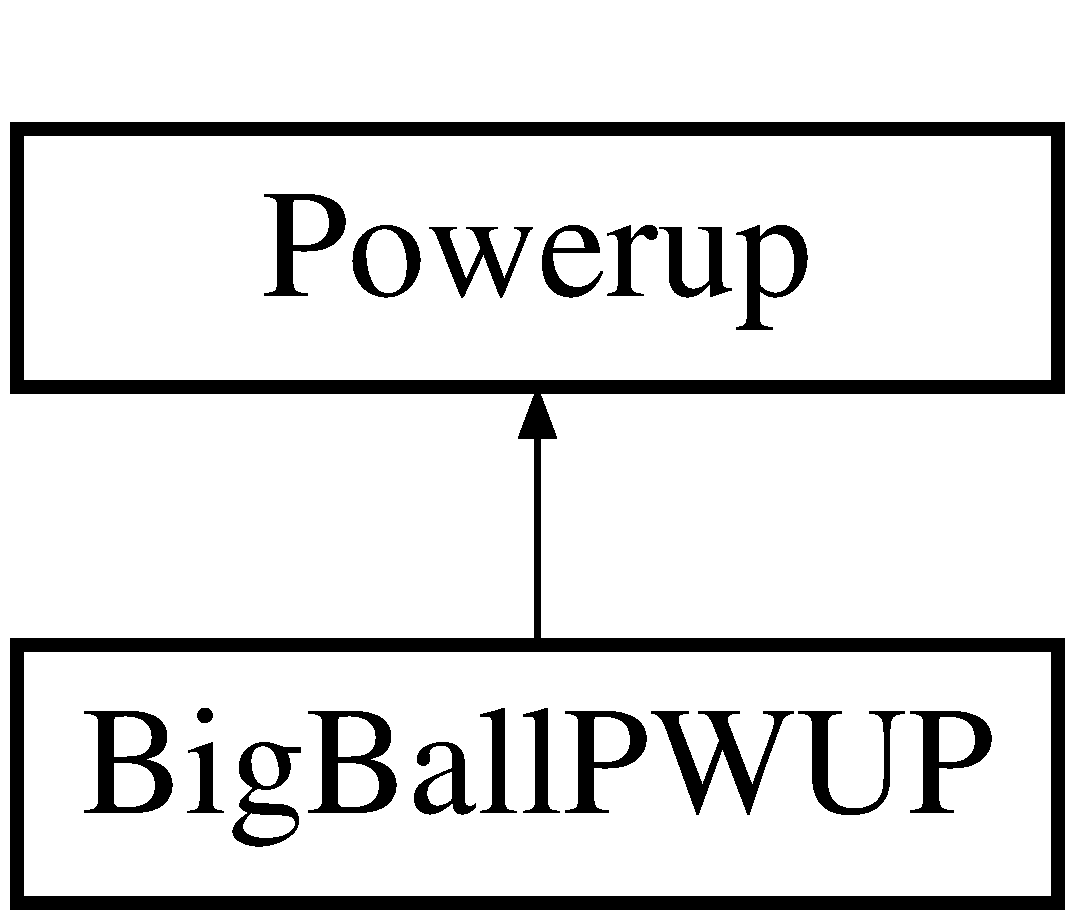
\includegraphics[height=2.000000cm]{class_big_ball_p_w_u_p}
\end{center}
\end{figure}
\subsection*{Public Member Functions}
\begin{DoxyCompactItemize}
\item 
\mbox{\Hypertarget{class_big_ball_p_w_u_p_aec72b39626dc1fae8315baf26c017905}\label{class_big_ball_p_w_u_p_aec72b39626dc1fae8315baf26c017905}} 
void \hyperlink{class_big_ball_p_w_u_p_aec72b39626dc1fae8315baf26c017905}{Collect} ()
\begin{DoxyCompactList}\small\item\em Calls effect the powerup has on player when collected. \end{DoxyCompactList}\item 
\mbox{\Hypertarget{class_big_ball_p_w_u_p_ad85fcac851119b10f530d2c3387eeeb7}\label{class_big_ball_p_w_u_p_ad85fcac851119b10f530d2c3387eeeb7}} 
{\bfseries Big\+Ball\+P\+W\+UP} (double xx, double yy)
\end{DoxyCompactItemize}
\subsection*{Additional Inherited Members}


\subsection{Detailed Description}
\hyperlink{class_powerup}{Powerup} making balls bigger. 

The documentation for this class was generated from the following file\+:\begin{DoxyCompactItemize}
\item 
Arkanoid/Powerup.\+h\end{DoxyCompactItemize}

\hypertarget{class_big_racket_p_w_u_p}{}\section{Big\+Racket\+P\+W\+UP Class Reference}
\label{class_big_racket_p_w_u_p}\index{Big\+Racket\+P\+W\+UP@{Big\+Racket\+P\+W\+UP}}


\hyperlink{class_powerup}{Powerup} incrasing the size of \hyperlink{class_racket}{Racket}.  




{\ttfamily \#include $<$Powerup.\+h$>$}

Inheritance diagram for Big\+Racket\+P\+W\+UP\+:\begin{figure}[H]
\begin{center}
\leavevmode
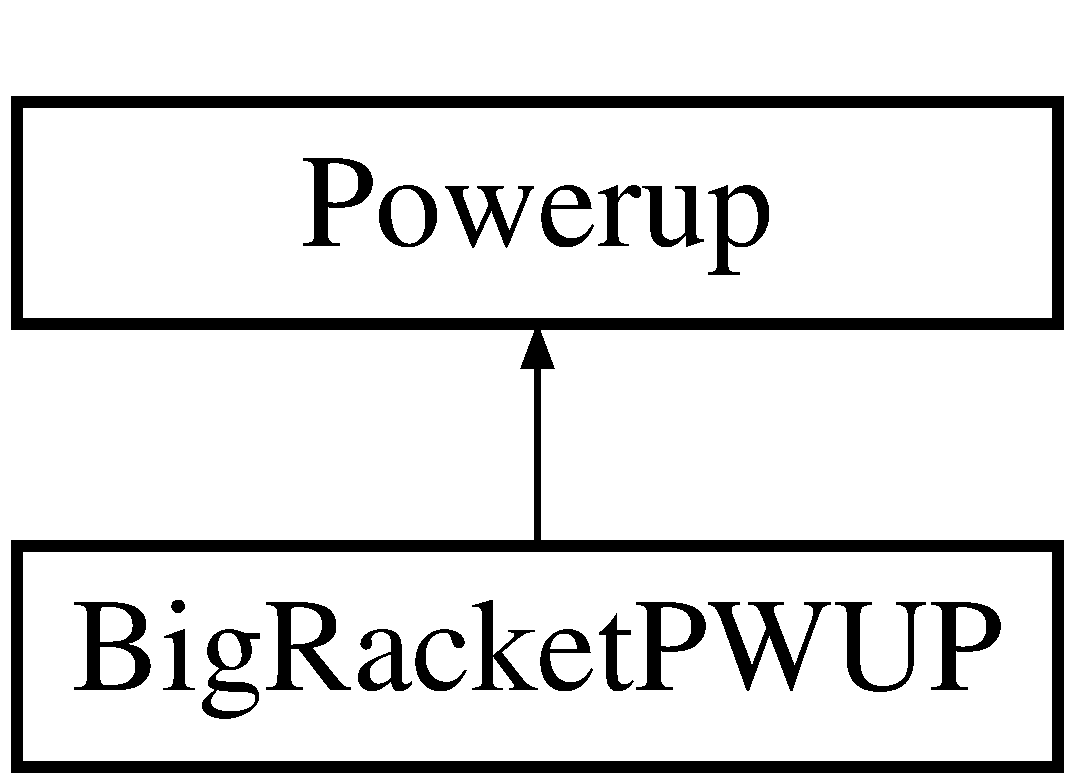
\includegraphics[height=2.000000cm]{class_big_racket_p_w_u_p}
\end{center}
\end{figure}
\subsection*{Public Member Functions}
\begin{DoxyCompactItemize}
\item 
\mbox{\Hypertarget{class_big_racket_p_w_u_p_aac3ff0b2045f8b7b044ad3237f9fb131}\label{class_big_racket_p_w_u_p_aac3ff0b2045f8b7b044ad3237f9fb131}} 
void \hyperlink{class_big_racket_p_w_u_p_aac3ff0b2045f8b7b044ad3237f9fb131}{Collect} ()
\begin{DoxyCompactList}\small\item\em Calls effect the powerup has on player when collected. \end{DoxyCompactList}\item 
\mbox{\Hypertarget{class_big_racket_p_w_u_p_a7bba1be71589caf1f8a5a3ca92b01485}\label{class_big_racket_p_w_u_p_a7bba1be71589caf1f8a5a3ca92b01485}} 
{\bfseries Big\+Racket\+P\+W\+UP} (double xx, double yy)
\end{DoxyCompactItemize}
\subsection*{Additional Inherited Members}


\subsection{Detailed Description}
\hyperlink{class_powerup}{Powerup} incrasing the size of \hyperlink{class_racket}{Racket}. 

The documentation for this class was generated from the following file\+:\begin{DoxyCompactItemize}
\item 
Arkanoid/Powerup.\+h\end{DoxyCompactItemize}

\hypertarget{class_block}{}\section{Block Class Reference}
\label{class_block}\index{Block@{Block}}


A class for a block.  




{\ttfamily \#include $<$Block.\+h$>$}

Inheritance diagram for Block\+:\begin{figure}[H]
\begin{center}
\leavevmode
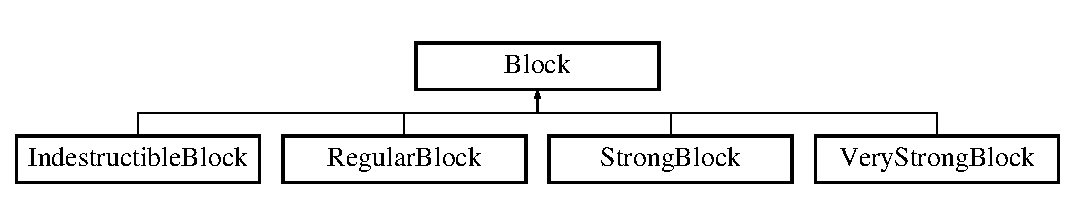
\includegraphics[height=2.000000cm]{class_block}
\end{center}
\end{figure}
\subsection*{Public Member Functions}
\begin{DoxyCompactItemize}
\item 
\mbox{\Hypertarget{class_block_ab79a68da4bbf6a22e1d91ac81d30ade8}\label{class_block_ab79a68da4bbf6a22e1d91ac81d30ade8}} 
{\bfseries Block} (char hlt=1, unsigned char r=0, unsigned char g=0, unsigned char b=0, unsigned char a=255)
\item 
void \hyperlink{class_block_aabe6fcade4ece2795cf4ada1f0241442}{Hit} (int=1)
\begin{DoxyCompactList}\small\item\em Records a block being hit, performs appropriate actions. \end{DoxyCompactList}\end{DoxyCompactItemize}
\subsection*{Public Attributes}
\begin{DoxyCompactItemize}
\item 
\hyperlink{struct_colour}{Colour} \hyperlink{class_block_acb5551f2233e2a97b9d9e7ab40590e33}{colour}
\begin{DoxyCompactList}\small\item\em \hyperlink{class_block}{Block} colour. \end{DoxyCompactList}\item 
\mbox{\Hypertarget{class_block_a13d0a6d225233353862fa5adcbadf661}\label{class_block_a13d0a6d225233353862fa5adcbadf661}} 
int \hyperlink{class_block_a13d0a6d225233353862fa5adcbadf661}{x}
\begin{DoxyCompactList}\small\item\em x coordinate of upper left corner. \end{DoxyCompactList}\item 
\mbox{\Hypertarget{class_block_a9328d6b6fcc9f9c019d091d87ceda41c}\label{class_block_a9328d6b6fcc9f9c019d091d87ceda41c}} 
int \hyperlink{class_block_a9328d6b6fcc9f9c019d091d87ceda41c}{y}
\begin{DoxyCompactList}\small\item\em y coordinate of upper left corner \end{DoxyCompactList}\item 
char \hyperlink{class_block_a5e2a1909ae2f2572cd75b2c38d3abddb}{health}
\begin{DoxyCompactList}\small\item\em \hyperlink{class_block}{Block} \char`\"{}hitpoints\char`\"{}. \end{DoxyCompactList}\end{DoxyCompactItemize}


\subsection{Detailed Description}
A class for a block. 

\subsection{Member Function Documentation}
\mbox{\Hypertarget{class_block_aabe6fcade4ece2795cf4ada1f0241442}\label{class_block_aabe6fcade4ece2795cf4ada1f0241442}} 
\index{Block@{Block}!Hit@{Hit}}
\index{Hit@{Hit}!Block@{Block}}
\subsubsection{\texorpdfstring{Hit()}{Hit()}}
{\footnotesize\ttfamily void Block\+::\+Hit (\begin{DoxyParamCaption}\item[{int}]{a = {\ttfamily 1} }\end{DoxyParamCaption})}



Records a block being hit, performs appropriate actions. 


\begin{DoxyParams}{Parameters}
{\em int} & Strength of a hit (power) \\
\hline
\end{DoxyParams}


\subsection{Member Data Documentation}
\mbox{\Hypertarget{class_block_acb5551f2233e2a97b9d9e7ab40590e33}\label{class_block_acb5551f2233e2a97b9d9e7ab40590e33}} 
\index{Block@{Block}!colour@{colour}}
\index{colour@{colour}!Block@{Block}}
\subsubsection{\texorpdfstring{colour}{colour}}
{\footnotesize\ttfamily \hyperlink{struct_colour}{Colour} Block\+::colour}



\hyperlink{class_block}{Block} colour. 

\hyperlink{class_block}{Block} colour, defined by struct in \hyperlink{_config_8h_source}{Config.\+h}. Contains of red, green, blue and alpha values, ranging from 0-\/255. \mbox{\Hypertarget{class_block_a5e2a1909ae2f2572cd75b2c38d3abddb}\label{class_block_a5e2a1909ae2f2572cd75b2c38d3abddb}} 
\index{Block@{Block}!health@{health}}
\index{health@{health}!Block@{Block}}
\subsubsection{\texorpdfstring{health}{health}}
{\footnotesize\ttfamily char Block\+::health}



\hyperlink{class_block}{Block} \char`\"{}hitpoints\char`\"{}. 

Defines how many times a block can be hit before disappearing. 

The documentation for this class was generated from the following files\+:\begin{DoxyCompactItemize}
\item 
Arkanoid/Block.\+h\item 
Arkanoid/Block.\+cpp\end{DoxyCompactItemize}

\hypertarget{struct_colour}{}\section{Colour Struct Reference}
\label{struct_colour}\index{Colour@{Colour}}
\subsection*{Public Attributes}
\begin{DoxyCompactItemize}
\item 
\mbox{\Hypertarget{struct_colour_ab0086c8227aa6faa9b1e5ec4f9a9e3ee}\label{struct_colour_ab0086c8227aa6faa9b1e5ec4f9a9e3ee}} 
unsigned char \hyperlink{struct_colour_ab0086c8227aa6faa9b1e5ec4f9a9e3ee}{r} = 0
\begin{DoxyCompactList}\small\item\em Red value. \end{DoxyCompactList}\item 
\mbox{\Hypertarget{struct_colour_a8f883cd0fbcae4be7611283083c4131f}\label{struct_colour_a8f883cd0fbcae4be7611283083c4131f}} 
unsigned char \hyperlink{struct_colour_a8f883cd0fbcae4be7611283083c4131f}{g} = 0
\begin{DoxyCompactList}\small\item\em Green value. \end{DoxyCompactList}\item 
\mbox{\Hypertarget{struct_colour_aca50ca8192a7538e0aaa2428ac84442a}\label{struct_colour_aca50ca8192a7538e0aaa2428ac84442a}} 
unsigned char \hyperlink{struct_colour_aca50ca8192a7538e0aaa2428ac84442a}{b} = 0
\begin{DoxyCompactList}\small\item\em Blue value. \end{DoxyCompactList}\item 
\mbox{\Hypertarget{struct_colour_a3dfbe5a33ed2f27365e2f22c669d29f2}\label{struct_colour_a3dfbe5a33ed2f27365e2f22c669d29f2}} 
unsigned char \hyperlink{struct_colour_a3dfbe5a33ed2f27365e2f22c669d29f2}{a} = 0
\begin{DoxyCompactList}\small\item\em Alpha value. \end{DoxyCompactList}\end{DoxyCompactItemize}


The documentation for this struct was generated from the following file\+:\begin{DoxyCompactItemize}
\item 
Arkanoid/Config.\+h\end{DoxyCompactItemize}

\hypertarget{class_enemy}{}\section{Enemy Class Reference}
\label{class_enemy}\index{Enemy@{Enemy}}


Main class for enemy, containing all variables and some default methods.  




{\ttfamily \#include $<$Enemy.\+h$>$}

Inheritance diagram for Enemy\+:\begin{figure}[H]
\begin{center}
\leavevmode
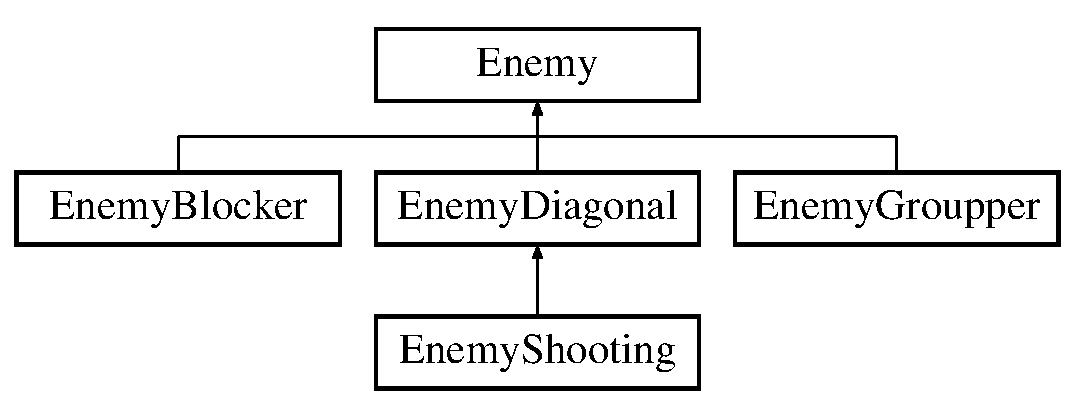
\includegraphics[height=3.000000cm]{class_enemy}
\end{center}
\end{figure}
\subsection*{Public Types}
\begin{DoxyCompactItemize}
\item 
\mbox{\Hypertarget{class_enemy_a98c2ee2c2081001de17a4bc9fa8da94f}\label{class_enemy_a98c2ee2c2081001de17a4bc9fa8da94f}} 
enum \hyperlink{class_enemy_a98c2ee2c2081001de17a4bc9fa8da94f}{Enemy\+Type} \{ {\bfseries D\+I\+A\+G\+O\+N\+AL}, 
{\bfseries S\+H\+O\+O\+T\+I\+N\+G\+D\+I\+A\+G\+O\+N\+AL}, 
{\bfseries G\+R\+O\+U\+P\+P\+ER}, 
{\bfseries B\+L\+O\+C\+K\+ER}
 \}\begin{DoxyCompactList}\small\item\em \hyperlink{class_enemy}{Enemy} type flag. \end{DoxyCompactList}
\end{DoxyCompactItemize}
\subsection*{Public Member Functions}
\begin{DoxyCompactItemize}
\item 
virtual void \hyperlink{class_enemy_ab7e37cac9017834db50d2aaf94e75034}{Move} (float time\+Step)
\begin{DoxyCompactList}\small\item\em Moves an enemy. Directly down for main class. \end{DoxyCompactList}\item 
\mbox{\Hypertarget{class_enemy_ac65dfd9eae4c84e890f9196941b18d62}\label{class_enemy_ac65dfd9eae4c84e890f9196941b18d62}} 
virtual void \hyperlink{class_enemy_ac65dfd9eae4c84e890f9196941b18d62}{Act} ()
\begin{DoxyCompactList}\small\item\em Performs an action enemy is supposed to do. Nothing for main class. \end{DoxyCompactList}\item 
\mbox{\Hypertarget{class_enemy_ac0eec4755e28c02688065f9657150ac3}\label{class_enemy_ac0eec4755e28c02688065f9657150ac3}} 
virtual \hyperlink{class_enemy_ac0eec4755e28c02688065f9657150ac3}{$\sim$\+Enemy} ()
\begin{DoxyCompactList}\small\item\em Virtual destructor for polimorphism. \end{DoxyCompactList}\end{DoxyCompactItemize}
\subsection*{Static Public Member Functions}
\begin{DoxyCompactItemize}
\item 
{\footnotesize template$<$class T $>$ }\\static std\+::vector$<$ \hyperlink{class_enemy}{Enemy} $\ast$ $>$ \hyperlink{class_enemy_a747d610b1a24386b9bd85c50132ffa98}{Get\+Inst} ()
\begin{DoxyCompactList}\small\item\em Function returning a vector of enemies of said type. \end{DoxyCompactList}\item 
{\footnotesize template$<$class T , class T2 , class... Rest$>$ }\\static std\+::vector$<$ \hyperlink{class_enemy}{Enemy} $\ast$ $>$ \hyperlink{class_enemy_a4c0528b6b7e94cfbceada5bd00f7193d}{Get\+Inst} ()
\begin{DoxyCompactList}\small\item\em Function returning a vector of enemies of said type. \end{DoxyCompactList}\item 
static void \hyperlink{class_enemy_afcf5991522f6f881e97b5910ac353633}{Move\+All} (float time\+Step)
\begin{DoxyCompactList}\small\item\em Calls specific Move methods on all enemies on enemy\+List vector. \end{DoxyCompactList}\end{DoxyCompactItemize}
\subsection*{Public Attributes}
\begin{DoxyCompactItemize}
\item 
\mbox{\Hypertarget{class_enemy_a05e9e91e87d6eae0da31cc6d78a0b43d}\label{class_enemy_a05e9e91e87d6eae0da31cc6d78a0b43d}} 
double \hyperlink{class_enemy_a05e9e91e87d6eae0da31cc6d78a0b43d}{x}
\begin{DoxyCompactList}\small\item\em \hyperlink{class_enemy}{Enemy} x coordinate. \end{DoxyCompactList}\item 
\mbox{\Hypertarget{class_enemy_a23d38ed46475359ad6a4e06d4dd49131}\label{class_enemy_a23d38ed46475359ad6a4e06d4dd49131}} 
double \hyperlink{class_enemy_a23d38ed46475359ad6a4e06d4dd49131}{y}
\begin{DoxyCompactList}\small\item\em \hyperlink{class_enemy}{Enemy} y coordinate. \end{DoxyCompactList}\item 
\mbox{\Hypertarget{class_enemy_af615681d1038587714a8552823e303d0}\label{class_enemy_af615681d1038587714a8552823e303d0}} 
double \hyperlink{class_enemy_af615681d1038587714a8552823e303d0}{Vx}
\begin{DoxyCompactList}\small\item\em \hyperlink{class_enemy}{Enemy} horizontal speed vector. \end{DoxyCompactList}\item 
\mbox{\Hypertarget{class_enemy_a60b9d71f1d711cb2d79787e4cce46046}\label{class_enemy_a60b9d71f1d711cb2d79787e4cce46046}} 
double \hyperlink{class_enemy_a60b9d71f1d711cb2d79787e4cce46046}{Vy}
\begin{DoxyCompactList}\small\item\em \hyperlink{class_enemy}{Enemy} vertical speed vector. \end{DoxyCompactList}\item 
int \hyperlink{class_enemy_aa8e17bc99723176548d71447e54cac73}{size}
\begin{DoxyCompactList}\small\item\em \hyperlink{class_enemy}{Enemy} size, in pixels. \end{DoxyCompactList}\item 
\mbox{\Hypertarget{class_enemy_a0be1b3814551bf2d43cbcd00a2c8134e}\label{class_enemy_a0be1b3814551bf2d43cbcd00a2c8134e}} 
double \hyperlink{class_enemy_a0be1b3814551bf2d43cbcd00a2c8134e}{bounceY}
\begin{DoxyCompactList}\small\item\em y coordinate value at which enemies will bounce off. \end{DoxyCompactList}\item 
\mbox{\Hypertarget{class_enemy_aebb86651c5be3c4e359a15b2832e5e4a}\label{class_enemy_aebb86651c5be3c4e359a15b2832e5e4a}} 
enum \hyperlink{class_enemy_a98c2ee2c2081001de17a4bc9fa8da94f}{Enemy\+::\+Enemy\+Type} {\bfseries enemy\+Type}
\item 
\hyperlink{struct_colour}{Colour} \hyperlink{class_enemy_a8fcd6954051e37e2ee89104e57145112}{colour}
\begin{DoxyCompactList}\small\item\em \hyperlink{class_enemy}{Enemy} colour. \end{DoxyCompactList}\end{DoxyCompactItemize}
\subsection*{Static Public Attributes}
\begin{DoxyCompactItemize}
\item 
\mbox{\Hypertarget{class_enemy_ad21b742c9768be0162f53d1beb212830}\label{class_enemy_ad21b742c9768be0162f53d1beb212830}} 
static std\+::vector$<$ \hyperlink{class_enemy}{Enemy} $\ast$ $>$ \hyperlink{class_enemy_ad21b742c9768be0162f53d1beb212830}{enemy\+List}
\begin{DoxyCompactList}\small\item\em List of enemies. \end{DoxyCompactList}\end{DoxyCompactItemize}
\subsection*{Protected Member Functions}
\begin{DoxyCompactItemize}
\item 
\mbox{\Hypertarget{class_enemy_a6124e0876e6ffd333ea69a246aecc993}\label{class_enemy_a6124e0876e6ffd333ea69a246aecc993}} 
{\bfseries Enemy} (int \hyperlink{class_enemy_a05e9e91e87d6eae0da31cc6d78a0b43d}{x}=0, int dirX=1)
\end{DoxyCompactItemize}


\subsection{Detailed Description}
Main class for enemy, containing all variables and some default methods. 

\subsection{Member Function Documentation}
\mbox{\Hypertarget{class_enemy_a747d610b1a24386b9bd85c50132ffa98}\label{class_enemy_a747d610b1a24386b9bd85c50132ffa98}} 
\index{Enemy@{Enemy}!Get\+Inst@{Get\+Inst}}
\index{Get\+Inst@{Get\+Inst}!Enemy@{Enemy}}
\subsubsection{\texorpdfstring{Get\+Inst()}{GetInst()}\hspace{0.1cm}{\footnotesize\ttfamily [1/2]}}
{\footnotesize\ttfamily template$<$class T $>$ \\
static std\+::vector$<$\hyperlink{class_enemy}{Enemy} $\ast$$>$ Enemy\+::\+Get\+Inst (\begin{DoxyParamCaption}{ }\end{DoxyParamCaption})\hspace{0.3cm}{\ttfamily [inline]}, {\ttfamily [static]}}



Function returning a vector of enemies of said type. 

Template function that is being called as\+: \hyperlink{class_enemy_a747d610b1a24386b9bd85c50132ffa98}{Get\+Inst$<$\+Enemy\+Type1$>$()}.

\begin{DoxyReturn}{Returns}
vector$<$\+Enemy $\ast$$>$ Vector of enemies of wanted types. 
\end{DoxyReturn}
\mbox{\Hypertarget{class_enemy_a4c0528b6b7e94cfbceada5bd00f7193d}\label{class_enemy_a4c0528b6b7e94cfbceada5bd00f7193d}} 
\index{Enemy@{Enemy}!Get\+Inst@{Get\+Inst}}
\index{Get\+Inst@{Get\+Inst}!Enemy@{Enemy}}
\subsubsection{\texorpdfstring{Get\+Inst()}{GetInst()}\hspace{0.1cm}{\footnotesize\ttfamily [2/2]}}
{\footnotesize\ttfamily template$<$class T , class T2 , class... Rest$>$ \\
static std\+::vector$<$\hyperlink{class_enemy}{Enemy} $\ast$$>$ Enemy\+::\+Get\+Inst (\begin{DoxyParamCaption}{ }\end{DoxyParamCaption})\hspace{0.3cm}{\ttfamily [inline]}, {\ttfamily [static]}}



Function returning a vector of enemies of said type. 

Template function that is being called as\+: \hyperlink{class_enemy_a747d610b1a24386b9bd85c50132ffa98}{Get\+Inst$<$\+Enemy\+Type1, Enemy\+Type2,...$>$()}.

\begin{DoxyReturn}{Returns}
vector$<$\+Enemy $\ast$$>$ Vector of enemies of wanted types. 
\end{DoxyReturn}
\mbox{\Hypertarget{class_enemy_ab7e37cac9017834db50d2aaf94e75034}\label{class_enemy_ab7e37cac9017834db50d2aaf94e75034}} 
\index{Enemy@{Enemy}!Move@{Move}}
\index{Move@{Move}!Enemy@{Enemy}}
\subsubsection{\texorpdfstring{Move()}{Move()}}
{\footnotesize\ttfamily void Enemy\+::\+Move (\begin{DoxyParamCaption}\item[{float}]{time\+Step }\end{DoxyParamCaption})\hspace{0.3cm}{\ttfamily [virtual]}}



Moves an enemy. Directly down for main class. 


\begin{DoxyParams}{Parameters}
{\em float} & time\+Step \\
\hline
\end{DoxyParams}


Reimplemented in \hyperlink{class_enemy_diagonal_aa33718254422fa69663e22c00e80d1d9}{Enemy\+Diagonal}.

\mbox{\Hypertarget{class_enemy_afcf5991522f6f881e97b5910ac353633}\label{class_enemy_afcf5991522f6f881e97b5910ac353633}} 
\index{Enemy@{Enemy}!Move\+All@{Move\+All}}
\index{Move\+All@{Move\+All}!Enemy@{Enemy}}
\subsubsection{\texorpdfstring{Move\+All()}{MoveAll()}}
{\footnotesize\ttfamily void Enemy\+::\+Move\+All (\begin{DoxyParamCaption}\item[{float}]{time\+Step }\end{DoxyParamCaption})\hspace{0.3cm}{\ttfamily [static]}}



Calls specific Move methods on all enemies on enemy\+List vector. 


\begin{DoxyParams}{Parameters}
{\em float} & time\+Step \\
\hline
\end{DoxyParams}


\subsection{Member Data Documentation}
\mbox{\Hypertarget{class_enemy_a8fcd6954051e37e2ee89104e57145112}\label{class_enemy_a8fcd6954051e37e2ee89104e57145112}} 
\index{Enemy@{Enemy}!colour@{colour}}
\index{colour@{colour}!Enemy@{Enemy}}
\subsubsection{\texorpdfstring{colour}{colour}}
{\footnotesize\ttfamily \hyperlink{struct_colour}{Colour} Enemy\+::colour}



\hyperlink{class_enemy}{Enemy} colour. 

\hyperlink{class_enemy}{Enemy} colour, defined by struct in \hyperlink{_config_8h_source}{Config.\+h}. Contains of red, green, blue and alpha values, ranging from 0-\/255. \mbox{\Hypertarget{class_enemy_aa8e17bc99723176548d71447e54cac73}\label{class_enemy_aa8e17bc99723176548d71447e54cac73}} 
\index{Enemy@{Enemy}!size@{size}}
\index{size@{size}!Enemy@{Enemy}}
\subsubsection{\texorpdfstring{size}{size}}
{\footnotesize\ttfamily int Enemy\+::size}



\hyperlink{class_enemy}{Enemy} size, in pixels. 

\hyperlink{class_enemy}{Enemy} is a ball, size defines the ball\textquotesingle{}s radius. 

The documentation for this class was generated from the following files\+:\begin{DoxyCompactItemize}
\item 
Arkanoid/Enemy.\+h\item 
Arkanoid/Enemy.\+cpp\end{DoxyCompactItemize}

\hypertarget{class_enemy_blocker}{}\section{Enemy\+Blocker Class Reference}
\label{class_enemy_blocker}\index{Enemy\+Blocker@{Enemy\+Blocker}}


\hyperlink{class_enemy}{Enemy} placing blocks.  




{\ttfamily \#include $<$Enemy.\+h$>$}

Inheritance diagram for Enemy\+Blocker\+:\begin{figure}[H]
\begin{center}
\leavevmode
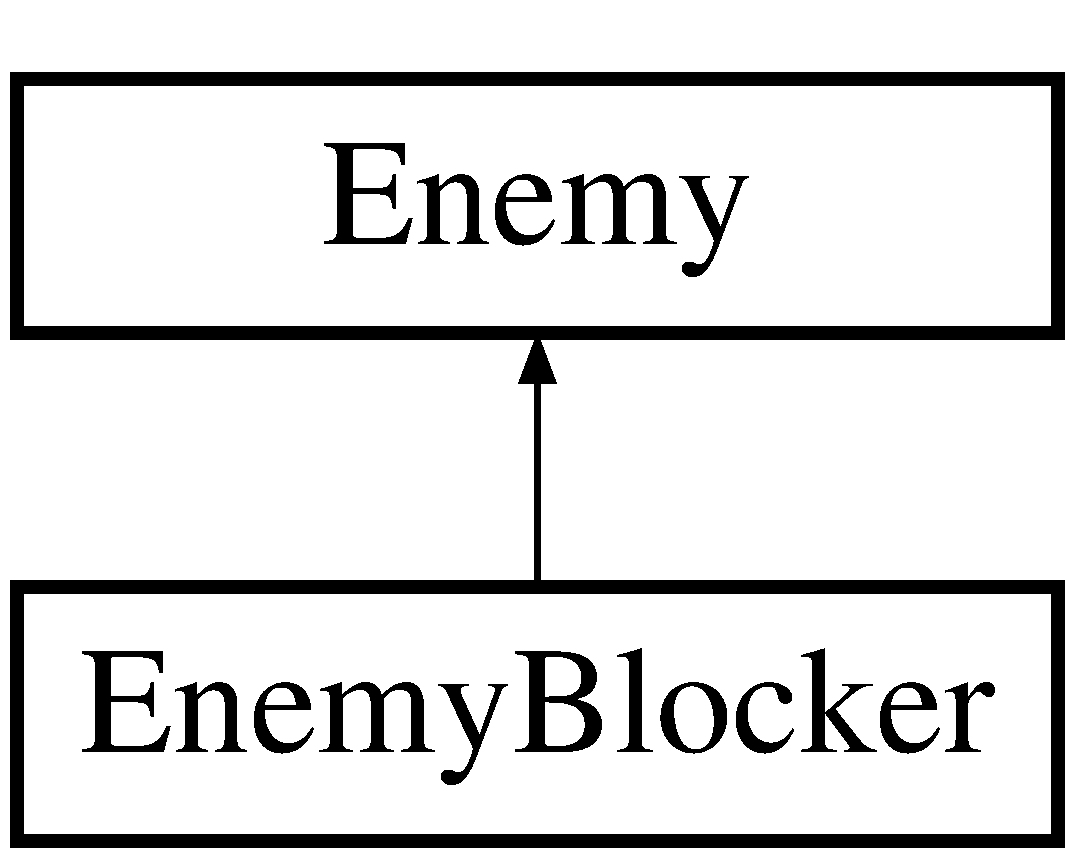
\includegraphics[height=2.000000cm]{class_enemy_blocker}
\end{center}
\end{figure}
\subsection*{Public Member Functions}
\begin{DoxyCompactItemize}
\item 
\mbox{\Hypertarget{class_enemy_blocker_a7e2eea95d73fb0ab5aa12f77ff1fbbb4}\label{class_enemy_blocker_a7e2eea95d73fb0ab5aa12f77ff1fbbb4}} 
{\bfseries Enemy\+Blocker} (int \hyperlink{class_enemy_a05e9e91e87d6eae0da31cc6d78a0b43d}{x}=0, int dirX=1)
\item 
\mbox{\Hypertarget{class_enemy_blocker_a9d56baea3bee22d819db3cc5be8c9e20}\label{class_enemy_blocker_a9d56baea3bee22d819db3cc5be8c9e20}} 
void \hyperlink{class_enemy_blocker_a9d56baea3bee22d819db3cc5be8c9e20}{Act} ()
\begin{DoxyCompactList}\small\item\em Places a regular block on its position, if no block exists. \end{DoxyCompactList}\end{DoxyCompactItemize}
\subsection*{Additional Inherited Members}


\subsection{Detailed Description}
\hyperlink{class_enemy}{Enemy} placing blocks. 

The documentation for this class was generated from the following files\+:\begin{DoxyCompactItemize}
\item 
Arkanoid/Enemy.\+h\item 
Arkanoid/Enemy.\+cpp\end{DoxyCompactItemize}

\hypertarget{class_enemy_diagonal}{}\section{Enemy\+Diagonal Class Reference}
\label{class_enemy_diagonal}\index{Enemy\+Diagonal@{Enemy\+Diagonal}}


\hyperlink{class_enemy}{Enemy} that moves in diagonal instead of directly down.  




{\ttfamily \#include $<$Enemy.\+h$>$}

Inheritance diagram for Enemy\+Diagonal\+:\begin{figure}[H]
\begin{center}
\leavevmode
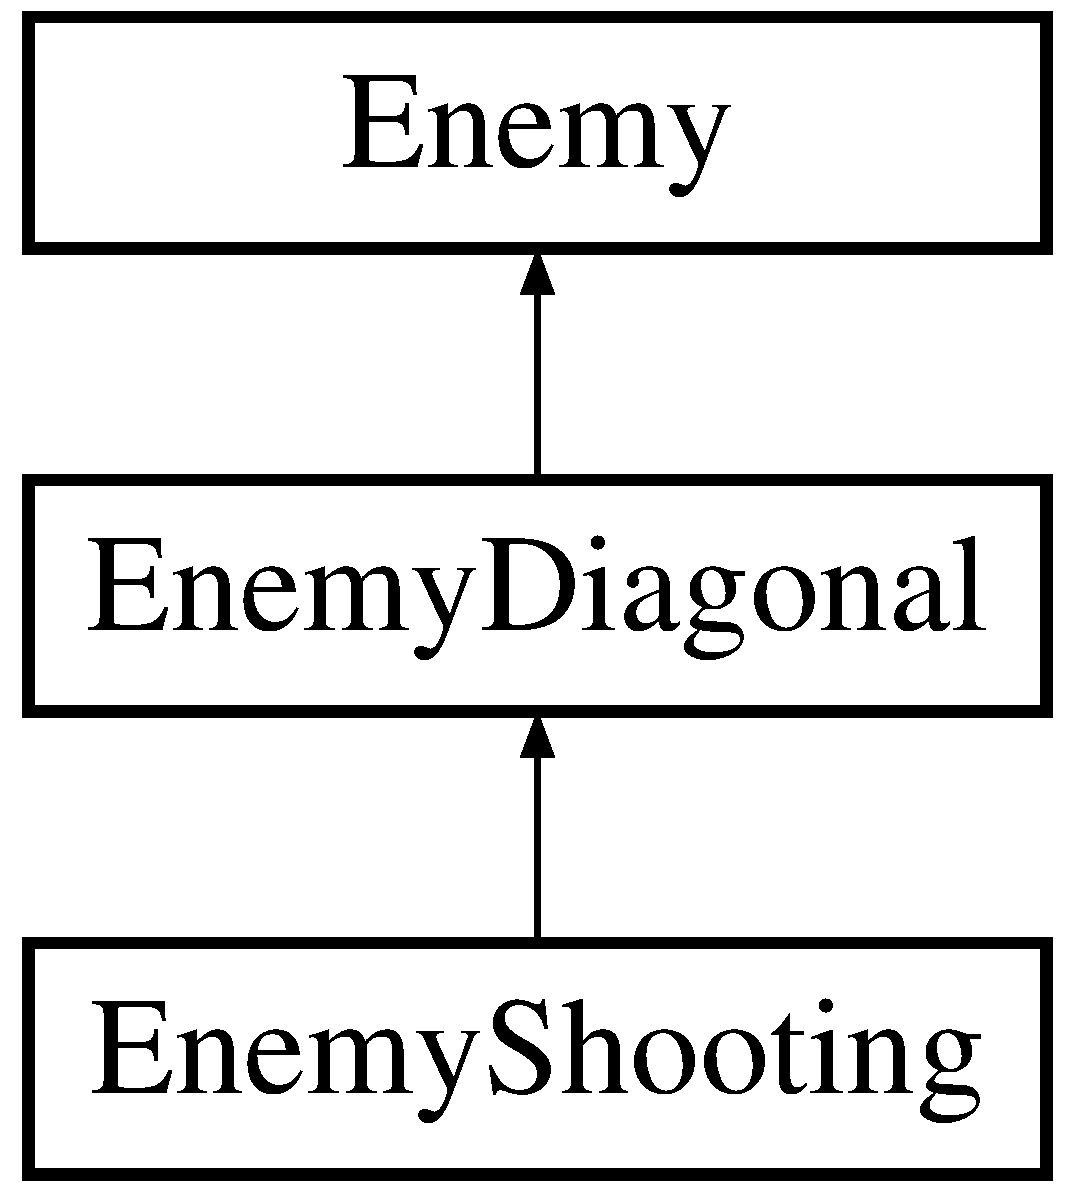
\includegraphics[height=3.000000cm]{class_enemy_diagonal}
\end{center}
\end{figure}
\subsection*{Public Member Functions}
\begin{DoxyCompactItemize}
\item 
\mbox{\Hypertarget{class_enemy_diagonal_a7c154e80303b201f5d5e28905f9d71f9}\label{class_enemy_diagonal_a7c154e80303b201f5d5e28905f9d71f9}} 
{\bfseries Enemy\+Diagonal} (int \hyperlink{class_enemy_a05e9e91e87d6eae0da31cc6d78a0b43d}{x}=0, int dirX=1)
\item 
\mbox{\Hypertarget{class_enemy_diagonal_aa33718254422fa69663e22c00e80d1d9}\label{class_enemy_diagonal_aa33718254422fa69663e22c00e80d1d9}} 
void \hyperlink{class_enemy_diagonal_aa33718254422fa69663e22c00e80d1d9}{Move} (float)
\begin{DoxyCompactList}\small\item\em Moves enemy in diagonal, much faster in horizontal axis. \end{DoxyCompactList}\end{DoxyCompactItemize}
\subsection*{Additional Inherited Members}


\subsection{Detailed Description}
\hyperlink{class_enemy}{Enemy} that moves in diagonal instead of directly down. 

The documentation for this class was generated from the following files\+:\begin{DoxyCompactItemize}
\item 
Arkanoid/Enemy.\+h\item 
Arkanoid/Enemy.\+cpp\end{DoxyCompactItemize}

\hypertarget{class_enemy_groupper}{}\section{Enemy\+Groupper Class Reference}
\label{class_enemy_groupper}\index{Enemy\+Groupper@{Enemy\+Groupper}}


\hyperlink{class_enemy}{Enemy} that changes all regular enemies of type \hyperlink{class_enemy_diagonal}{Enemy\+Diagonal} into \hyperlink{class_enemy_shooting}{Enemy\+Shooting} (in its vincinity).  




{\ttfamily \#include $<$Enemy.\+h$>$}

Inheritance diagram for Enemy\+Groupper\+:\begin{figure}[H]
\begin{center}
\leavevmode
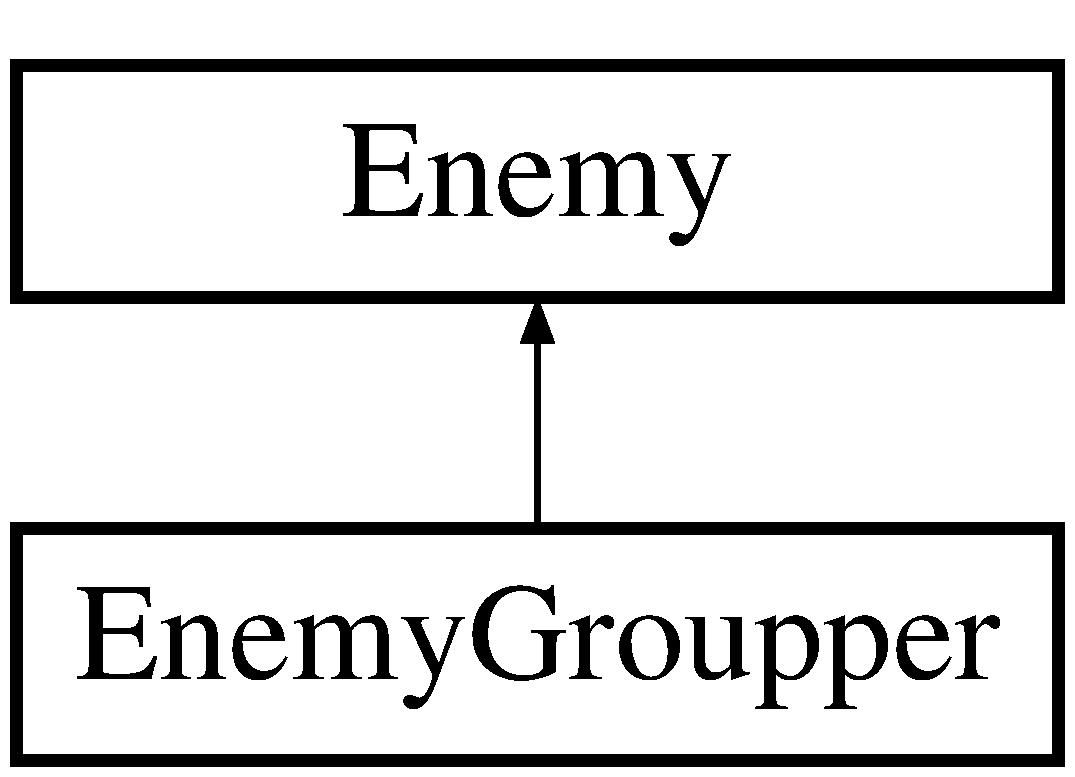
\includegraphics[height=2.000000cm]{class_enemy_groupper}
\end{center}
\end{figure}
\subsection*{Public Member Functions}
\begin{DoxyCompactItemize}
\item 
\mbox{\Hypertarget{class_enemy_groupper_a323134bc15ad87e603e75362e71ff7a8}\label{class_enemy_groupper_a323134bc15ad87e603e75362e71ff7a8}} 
{\bfseries Enemy\+Groupper} (int \hyperlink{class_enemy_a05e9e91e87d6eae0da31cc6d78a0b43d}{x}=0, int dirX=1)
\item 
\mbox{\Hypertarget{class_enemy_groupper_a2c322b4ff5a8d0540d7f20cb3e60c387}\label{class_enemy_groupper_a2c322b4ff5a8d0540d7f20cb3e60c387}} 
void \hyperlink{class_enemy_groupper_a2c322b4ff5a8d0540d7f20cb3e60c387}{Act} ()
\begin{DoxyCompactList}\small\item\em Looks for \hyperlink{class_enemy_diagonal}{Enemy\+Diagonal} nearby and converts them to \hyperlink{class_enemy_shooting}{Enemy\+Shooting},. \end{DoxyCompactList}\end{DoxyCompactItemize}
\subsection*{Additional Inherited Members}


\subsection{Detailed Description}
\hyperlink{class_enemy}{Enemy} that changes all regular enemies of type \hyperlink{class_enemy_diagonal}{Enemy\+Diagonal} into \hyperlink{class_enemy_shooting}{Enemy\+Shooting} (in its vincinity). 

The documentation for this class was generated from the following files\+:\begin{DoxyCompactItemize}
\item 
Arkanoid/Enemy.\+h\item 
Arkanoid/Enemy.\+cpp\end{DoxyCompactItemize}

\hypertarget{class_enemy_shooting}{}\section{Enemy\+Shooting Class Reference}
\label{class_enemy_shooting}\index{Enemy\+Shooting@{Enemy\+Shooting}}


\hyperlink{class_enemy_diagonal}{Enemy\+Diagonal} that fires missiles.  




{\ttfamily \#include $<$Enemy.\+h$>$}

Inheritance diagram for Enemy\+Shooting\+:\begin{figure}[H]
\begin{center}
\leavevmode
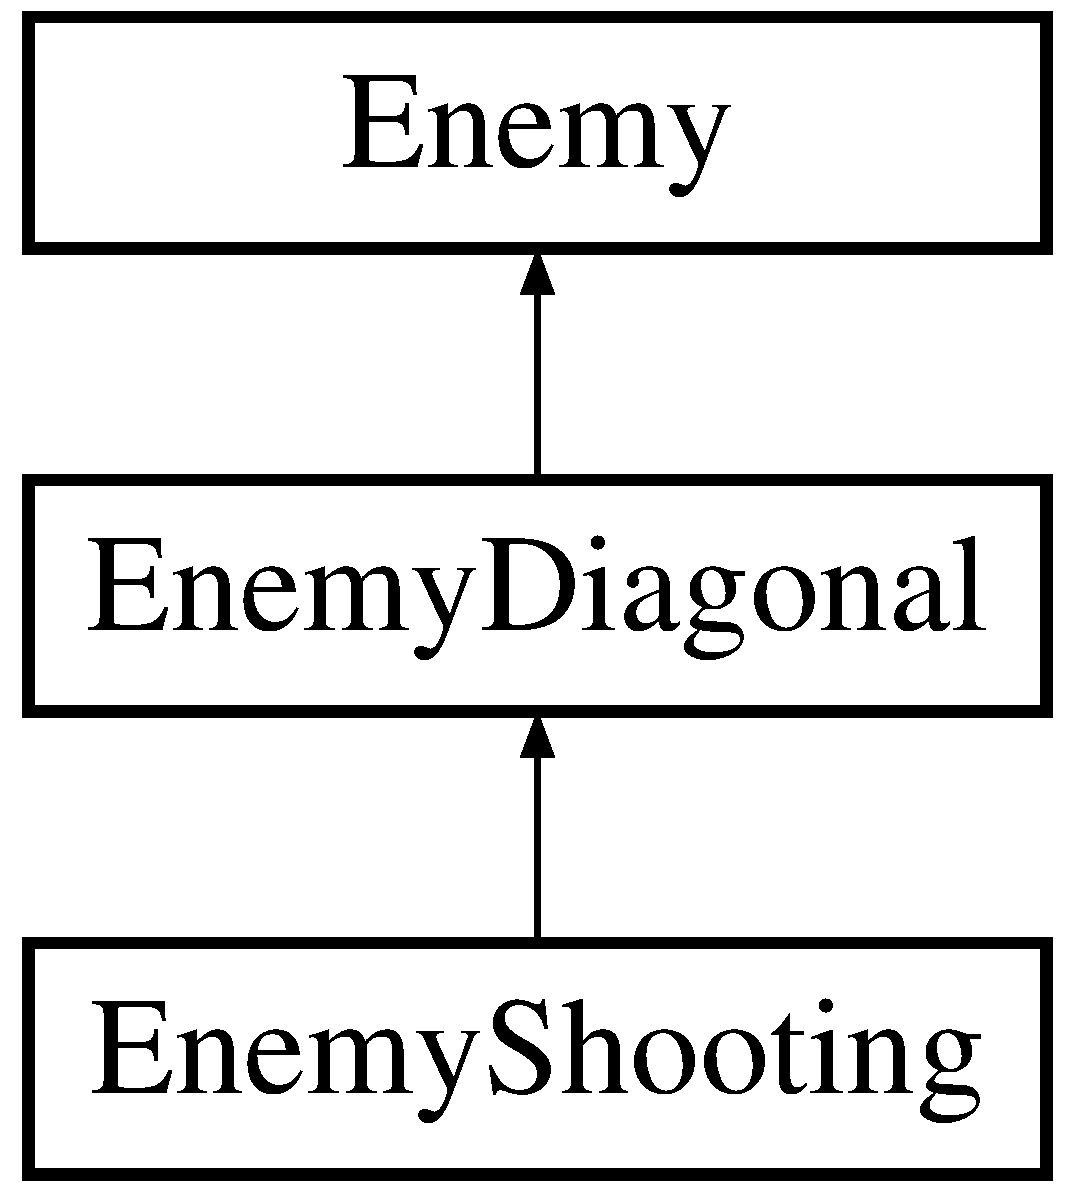
\includegraphics[height=3.000000cm]{class_enemy_shooting}
\end{center}
\end{figure}
\subsection*{Public Member Functions}
\begin{DoxyCompactItemize}
\item 
\mbox{\Hypertarget{class_enemy_shooting_aa66f1d05c29246f1904e8ebf9e25ca65}\label{class_enemy_shooting_aa66f1d05c29246f1904e8ebf9e25ca65}} 
{\bfseries Enemy\+Shooting} (int \hyperlink{class_enemy_a05e9e91e87d6eae0da31cc6d78a0b43d}{x}=0, int dirX=1)
\item 
\mbox{\Hypertarget{class_enemy_shooting_abee255a2e67785aab7bf7f6fb67d4ec9}\label{class_enemy_shooting_abee255a2e67785aab7bf7f6fb67d4ec9}} 
{\bfseries Enemy\+Shooting} (\hyperlink{class_enemy}{Enemy} \&)
\item 
\mbox{\Hypertarget{class_enemy_shooting_ad1b0698807426c5d5e337aca745111dc}\label{class_enemy_shooting_ad1b0698807426c5d5e337aca745111dc}} 
void \hyperlink{class_enemy_shooting_ad1b0698807426c5d5e337aca745111dc}{Act} ()
\begin{DoxyCompactList}\small\item\em Fires a \hyperlink{class_missile}{Missile}. \end{DoxyCompactList}\end{DoxyCompactItemize}
\subsection*{Additional Inherited Members}


\subsection{Detailed Description}
\hyperlink{class_enemy_diagonal}{Enemy\+Diagonal} that fires missiles. 

The documentation for this class was generated from the following files\+:\begin{DoxyCompactItemize}
\item 
Arkanoid/Enemy.\+h\item 
Arkanoid/Enemy.\+cpp\end{DoxyCompactItemize}

\hypertarget{class_extra_live_p_w_u_p}{}\section{Extra\+Live\+P\+W\+UP Class Reference}
\label{class_extra_live_p_w_u_p}\index{Extra\+Live\+P\+W\+UP@{Extra\+Live\+P\+W\+UP}}


\hyperlink{class_powerup}{Powerup} incrasing the live amount.  




{\ttfamily \#include $<$Powerup.\+h$>$}

Inheritance diagram for Extra\+Live\+P\+W\+UP\+:\begin{figure}[H]
\begin{center}
\leavevmode
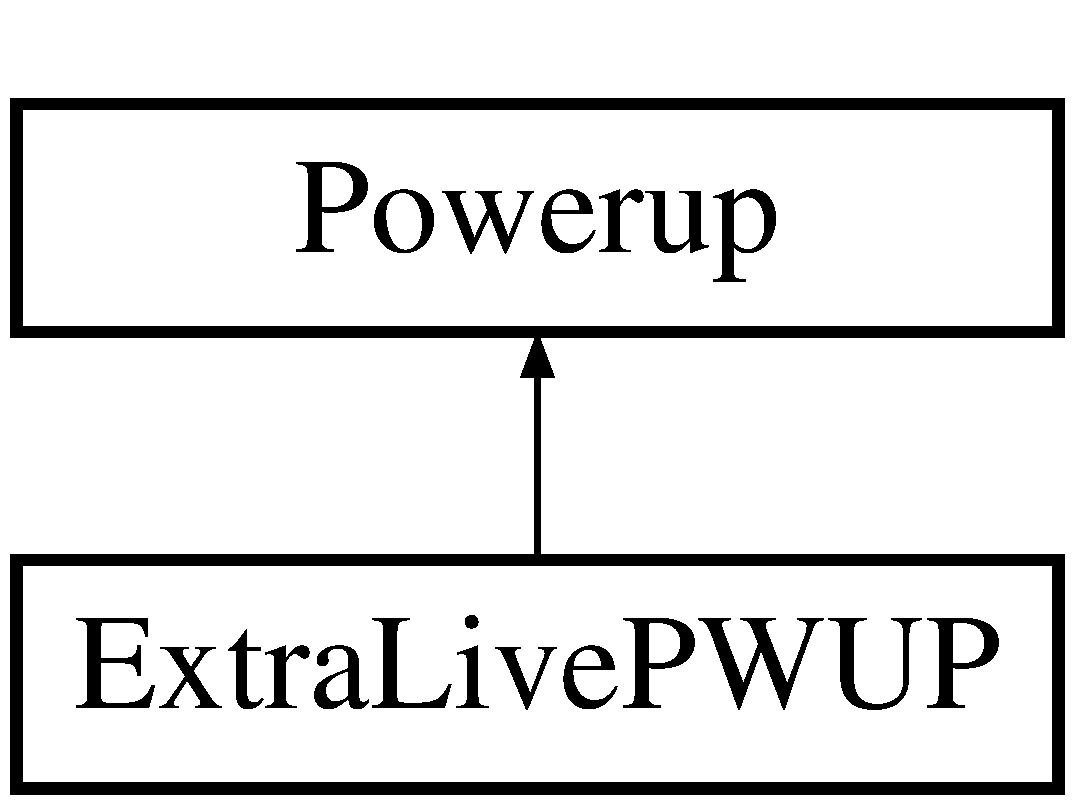
\includegraphics[height=2.000000cm]{class_extra_live_p_w_u_p}
\end{center}
\end{figure}
\subsection*{Public Member Functions}
\begin{DoxyCompactItemize}
\item 
\mbox{\Hypertarget{class_extra_live_p_w_u_p_add3e2d84928abe015534dbc8768158c8}\label{class_extra_live_p_w_u_p_add3e2d84928abe015534dbc8768158c8}} 
void \hyperlink{class_extra_live_p_w_u_p_add3e2d84928abe015534dbc8768158c8}{Collect} ()
\begin{DoxyCompactList}\small\item\em Calls effect the powerup has on player when collected. \end{DoxyCompactList}\item 
\mbox{\Hypertarget{class_extra_live_p_w_u_p_ac3f06611f79a518dd883c255e81a979b}\label{class_extra_live_p_w_u_p_ac3f06611f79a518dd883c255e81a979b}} 
{\bfseries Extra\+Live\+P\+W\+UP} (double xx, double yy)
\end{DoxyCompactItemize}
\subsection*{Additional Inherited Members}


\subsection{Detailed Description}
\hyperlink{class_powerup}{Powerup} incrasing the live amount. 

The documentation for this class was generated from the following file\+:\begin{DoxyCompactItemize}
\item 
Arkanoid/Powerup.\+h\end{DoxyCompactItemize}

\hypertarget{class_fast_ball_p_w_u_p}{}\section{Fast\+Ball\+P\+W\+UP Class Reference}
\label{class_fast_ball_p_w_u_p}\index{Fast\+Ball\+P\+W\+UP@{Fast\+Ball\+P\+W\+UP}}


\hyperlink{class_powerup}{Powerup} incrasing the speed of balls.  




{\ttfamily \#include $<$Powerup.\+h$>$}

Inheritance diagram for Fast\+Ball\+P\+W\+UP\+:\begin{figure}[H]
\begin{center}
\leavevmode
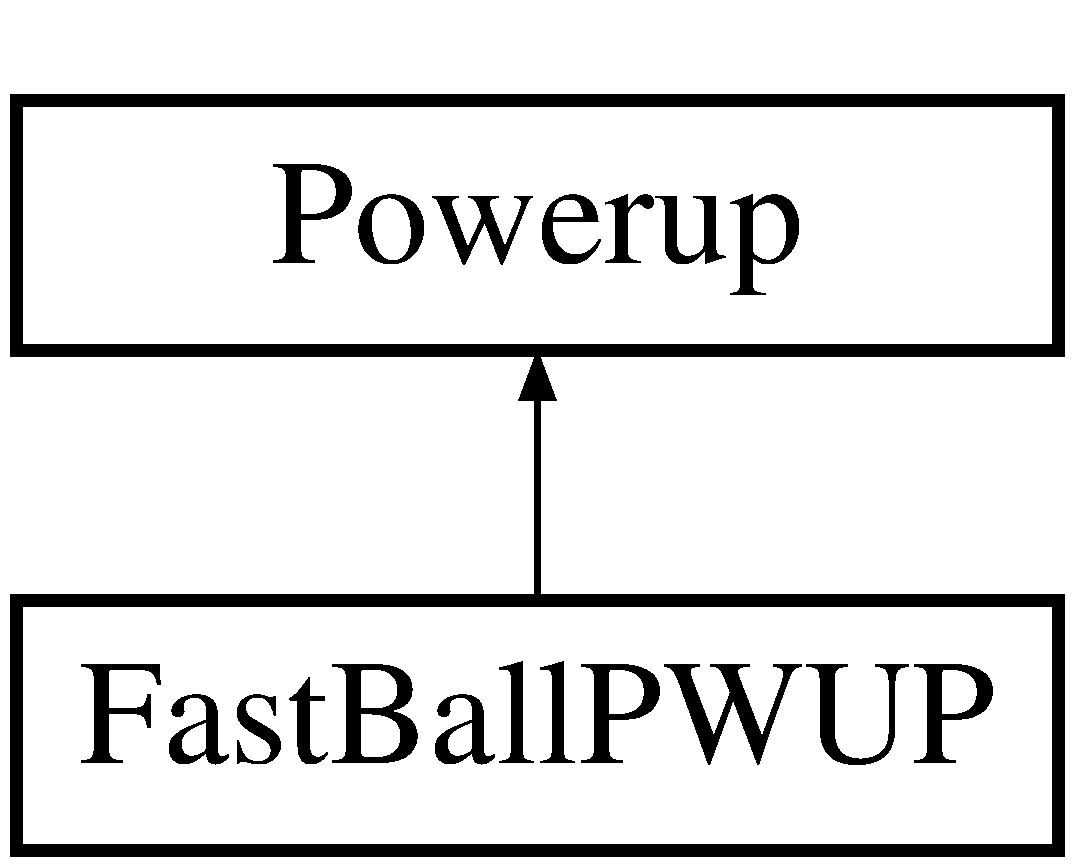
\includegraphics[height=2.000000cm]{class_fast_ball_p_w_u_p}
\end{center}
\end{figure}
\subsection*{Public Member Functions}
\begin{DoxyCompactItemize}
\item 
\mbox{\Hypertarget{class_fast_ball_p_w_u_p_a35493f4157c289174752a6b16f1b8fc2}\label{class_fast_ball_p_w_u_p_a35493f4157c289174752a6b16f1b8fc2}} 
void \hyperlink{class_fast_ball_p_w_u_p_a35493f4157c289174752a6b16f1b8fc2}{Collect} ()
\begin{DoxyCompactList}\small\item\em Calls effect the powerup has on player when collected. \end{DoxyCompactList}\item 
\mbox{\Hypertarget{class_fast_ball_p_w_u_p_acbb7e5b3a7febc34b7f4577971c6552c}\label{class_fast_ball_p_w_u_p_acbb7e5b3a7febc34b7f4577971c6552c}} 
{\bfseries Fast\+Ball\+P\+W\+UP} (double xx, double yy)
\end{DoxyCompactItemize}
\subsection*{Additional Inherited Members}


\subsection{Detailed Description}
\hyperlink{class_powerup}{Powerup} incrasing the speed of balls. 

The documentation for this class was generated from the following file\+:\begin{DoxyCompactItemize}
\item 
Arkanoid/Powerup.\+h\end{DoxyCompactItemize}

\hypertarget{class_file_op}{}\section{File\+Op Class Reference}
\label{class_file_op}\index{File\+Op@{File\+Op}}


Class containing methods for operations between player and files.  




{\ttfamily \#include $<$Player.\+h$>$}

\subsection*{Static Protected Member Functions}
\begin{DoxyCompactItemize}
\item 
static int \hyperlink{class_file_op_ad0b6c298ae4ba9a9e17c70b432977bcc}{Load\+Level} (int n)
\begin{DoxyCompactList}\small\item\em Loads a level from J\+S\+ON file. \end{DoxyCompactList}\item 
\mbox{\Hypertarget{class_file_op_a7e8d42a9a08831340f0c26bd641153e2}\label{class_file_op_a7e8d42a9a08831340f0c26bd641153e2}} 
static \hyperlink{struct_save_data}{Save\+Data} \hyperlink{class_file_op_a7e8d42a9a08831340f0c26bd641153e2}{Load\+Game} ()
\begin{DoxyCompactList}\small\item\em Loads a savefile. \end{DoxyCompactList}\item 
\mbox{\Hypertarget{class_file_op_a727f9a9fd9700f753afeda9c0d1e04d8}\label{class_file_op_a727f9a9fd9700f753afeda9c0d1e04d8}} 
static int \hyperlink{class_file_op_a727f9a9fd9700f753afeda9c0d1e04d8}{Save\+Game} (\hyperlink{struct_save_data}{Save\+Data})
\begin{DoxyCompactList}\small\item\em Saves the game to file. \end{DoxyCompactList}\end{DoxyCompactItemize}


\subsection{Detailed Description}
Class containing methods for operations between player and files. 

\subsection{Member Function Documentation}
\mbox{\Hypertarget{class_file_op_ad0b6c298ae4ba9a9e17c70b432977bcc}\label{class_file_op_ad0b6c298ae4ba9a9e17c70b432977bcc}} 
\index{File\+Op@{File\+Op}!Load\+Level@{Load\+Level}}
\index{Load\+Level@{Load\+Level}!File\+Op@{File\+Op}}
\subsubsection{\texorpdfstring{Load\+Level()}{LoadLevel()}}
{\footnotesize\ttfamily int File\+Op\+::\+Load\+Level (\begin{DoxyParamCaption}\item[{int}]{n }\end{DoxyParamCaption})\hspace{0.3cm}{\ttfamily [static]}, {\ttfamily [protected]}}



Loads a level from J\+S\+ON file. 


\begin{DoxyParams}{Parameters}
{\em int} & Number of level to be loaded.\\
\hline
\end{DoxyParams}
\begin{DoxyReturn}{Returns}
int success flag. 
\end{DoxyReturn}


The documentation for this class was generated from the following files\+:\begin{DoxyCompactItemize}
\item 
Arkanoid/Player.\+h\item 
Arkanoid/Player.\+cpp\end{DoxyCompactItemize}

\hypertarget{class_game_field}{}\section{Game\+Field Class Reference}
\label{class_game_field}\index{Game\+Field@{Game\+Field}}


A class containing most elements needed to calculate behaviour.  




{\ttfamily \#include $<$Game\+Field.\+h$>$}

\subsection*{Public Member Functions}
\begin{DoxyCompactItemize}
\item 
int \hyperlink{class_game_field_ac5ab828d2d8dbabc75dedfc8f699a42c}{Add\+Block} (int, int, Block\+Type, \hyperlink{struct_colour}{Colour}=\{ 0, 0, 0, 0 \})
\begin{DoxyCompactList}\small\item\em Adds a block to the matrix -\/ gamefield. \end{DoxyCompactList}\item 
\mbox{\Hypertarget{class_game_field_a507ffac780fc8775a56e5e7af44c8960}\label{class_game_field_a507ffac780fc8775a56e5e7af44c8960}} 
void \hyperlink{class_game_field_a507ffac780fc8775a56e5e7af44c8960}{Purge\+Blocks} ()
\begin{DoxyCompactList}\small\item\em Purge the matrix and vector. \end{DoxyCompactList}\item 
\mbox{\Hypertarget{class_game_field_ad408237f35b181d21dd5fa1b473c8ca8}\label{class_game_field_ad408237f35b181d21dd5fa1b473c8ca8}} 
bool \hyperlink{class_game_field_ad408237f35b181d21dd5fa1b473c8ca8}{Is\+Clear} ()
\begin{DoxyCompactList}\small\item\em Checks if board is clear. \end{DoxyCompactList}\end{DoxyCompactItemize}
\subsection*{Static Public Member Functions}
\begin{DoxyCompactItemize}
\item 
\mbox{\Hypertarget{class_game_field_ad487d606fc86f967f58ec65d85684058}\label{class_game_field_ad487d606fc86f967f58ec65d85684058}} 
static \hyperlink{class_game_field}{Game\+Field} \& {\bfseries get\+Instance} ()
\end{DoxyCompactItemize}
\subsection*{Public Attributes}
\begin{DoxyCompactItemize}
\item 
\hyperlink{class_block}{Block} $\ast$ \hyperlink{class_game_field_a5b6cafcddfb83370e71363fc7b46a6f7}{block\+Matrix} \mbox{[}F\+I\+E\+L\+D\+\_\+\+W\+I\+D\+TH\mbox{]}\mbox{[}F\+I\+E\+L\+D\+\_\+\+H\+E\+I\+G\+HT\mbox{]}
\begin{DoxyCompactList}\small\item\em Matrix to roughly know block location. \end{DoxyCompactList}\end{DoxyCompactItemize}
\subsection*{Static Public Attributes}
\begin{DoxyCompactItemize}
\item 
\mbox{\Hypertarget{class_game_field_a993a881f800ac9c73cea3060eea16aea}\label{class_game_field_a993a881f800ac9c73cea3060eea16aea}} 
static std\+::vector$<$ \hyperlink{class_block}{Block} $\ast$ $>$ \hyperlink{class_game_field_a993a881f800ac9c73cea3060eea16aea}{block\+List}
\begin{DoxyCompactList}\small\item\em Vector to keep track of blocks. \end{DoxyCompactList}\item 
\mbox{\Hypertarget{class_game_field_a73fb44513fda2f45f7ddfe589222067c}\label{class_game_field_a73fb44513fda2f45f7ddfe589222067c}} 
static std\+::vector$<$ \hyperlink{class_powerup}{Powerup} $\ast$ $>$ \hyperlink{class_game_field_a73fb44513fda2f45f7ddfe589222067c}{powerup\+List}
\begin{DoxyCompactList}\small\item\em Vector to keep track of powerups. \end{DoxyCompactList}\end{DoxyCompactItemize}


\subsection{Detailed Description}
A class containing most elements needed to calculate behaviour. 

\subsection{Member Function Documentation}
\mbox{\Hypertarget{class_game_field_ac5ab828d2d8dbabc75dedfc8f699a42c}\label{class_game_field_ac5ab828d2d8dbabc75dedfc8f699a42c}} 
\index{Game\+Field@{Game\+Field}!Add\+Block@{Add\+Block}}
\index{Add\+Block@{Add\+Block}!Game\+Field@{Game\+Field}}
\subsubsection{\texorpdfstring{Add\+Block()}{AddBlock()}}
{\footnotesize\ttfamily int Game\+Field\+::\+Add\+Block (\begin{DoxyParamCaption}\item[{int}]{x,  }\item[{int}]{y,  }\item[{Block\+Type}]{type,  }\item[{\hyperlink{struct_colour}{Colour}}]{colour = {\ttfamily \{~0,0,0,0~\}} }\end{DoxyParamCaption})}



Adds a block to the matrix -\/ gamefield. 


\begin{DoxyParams}{Parameters}
{\em int} & X coordinate in matrix \\
\hline
{\em int} & Y coordinate in matrix \\
\hline
{\em Block\+Type} & Block\+Type of the block to be placed \\
\hline
{\em \hyperlink{struct_colour}{Colour}} & \hyperlink{struct_colour}{Colour} of the block to be palced\\
\hline
\end{DoxyParams}
\begin{DoxyReturn}{Returns}
1 If placed successfully 

0 If block exists in that spot 
\end{DoxyReturn}


\subsection{Member Data Documentation}
\mbox{\Hypertarget{class_game_field_a5b6cafcddfb83370e71363fc7b46a6f7}\label{class_game_field_a5b6cafcddfb83370e71363fc7b46a6f7}} 
\index{Game\+Field@{Game\+Field}!block\+Matrix@{block\+Matrix}}
\index{block\+Matrix@{block\+Matrix}!Game\+Field@{Game\+Field}}
\subsubsection{\texorpdfstring{block\+Matrix}{blockMatrix}}
{\footnotesize\ttfamily \hyperlink{class_block}{Block}$\ast$ Game\+Field\+::block\+Matrix\mbox{[}F\+I\+E\+L\+D\+\_\+\+W\+I\+D\+TH\mbox{]}\mbox{[}F\+I\+E\+L\+D\+\_\+\+H\+E\+I\+G\+HT\mbox{]}}



Matrix to roughly know block location. 

Used to check if block is alredy placed in one place, to avoid multiple blocks on the same tile. 

The documentation for this class was generated from the following files\+:\begin{DoxyCompactItemize}
\item 
Arkanoid/Game\+Field.\+h\item 
Arkanoid/Game\+Field.\+cpp\end{DoxyCompactItemize}

\hypertarget{class_indestructible_block}{}\section{Indestructible\+Block Class Reference}
\label{class_indestructible_block}\index{Indestructible\+Block@{Indestructible\+Block}}


\hyperlink{class_block}{Block} that cannot be destroyed.  




{\ttfamily \#include $<$Block.\+h$>$}

Inheritance diagram for Indestructible\+Block\+:\begin{figure}[H]
\begin{center}
\leavevmode
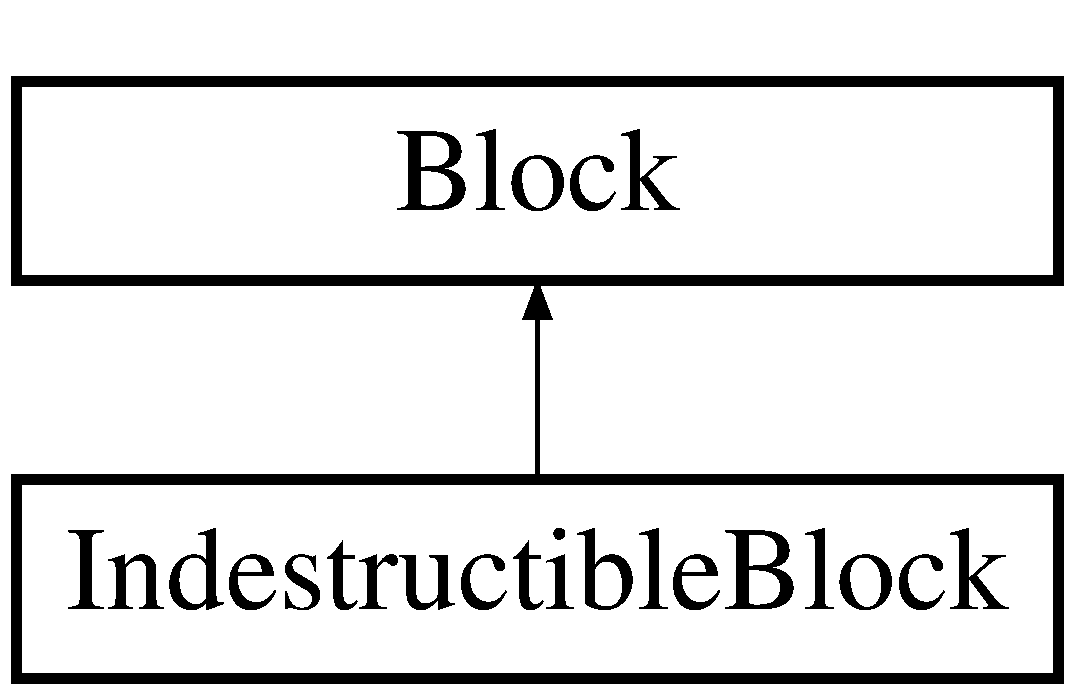
\includegraphics[height=2.000000cm]{class_indestructible_block}
\end{center}
\end{figure}
\subsection*{Public Member Functions}
\begin{DoxyCompactItemize}
\item 
\mbox{\Hypertarget{class_indestructible_block_afc762bad01f64e0b8826aab7691c5df4}\label{class_indestructible_block_afc762bad01f64e0b8826aab7691c5df4}} 
{\bfseries Indestructible\+Block} (char hlt=I\+N\+D\+E\+S\+T\+R\+U\+C\+T\+I\+B\+L\+E\+\_\+\+B\+L\+O\+C\+K\+\_\+\+H\+E\+A\+L\+TH, unsigned char r=200, unsigned char g=200, unsigned char b=200, unsigned char a=255)
\end{DoxyCompactItemize}
\subsection*{Additional Inherited Members}


\subsection{Detailed Description}
\hyperlink{class_block}{Block} that cannot be destroyed. 

The documentation for this class was generated from the following file\+:\begin{DoxyCompactItemize}
\item 
Arkanoid/Block.\+h\end{DoxyCompactItemize}

\hypertarget{class_l_texture}{}\section{L\+Texture Class Reference}
\label{class_l_texture}\index{L\+Texture@{L\+Texture}}


Texture wrapper class.  




{\ttfamily \#include $<$Render.\+h$>$}

\subsection*{Public Member Functions}
\begin{DoxyCompactItemize}
\item 
\mbox{\Hypertarget{class_l_texture_a12fbc9278f97388cce5ce18863b462ff}\label{class_l_texture_a12fbc9278f97388cce5ce18863b462ff}} 
\hyperlink{class_l_texture_a12fbc9278f97388cce5ce18863b462ff}{L\+Texture} ()
\begin{DoxyCompactList}\small\item\em Initializes variables. \end{DoxyCompactList}\item 
\mbox{\Hypertarget{class_l_texture_a49cfe57c36e58ad99c1ea73fc274b77b}\label{class_l_texture_a49cfe57c36e58ad99c1ea73fc274b77b}} 
\hyperlink{class_l_texture_a49cfe57c36e58ad99c1ea73fc274b77b}{$\sim$\+L\+Texture} ()
\begin{DoxyCompactList}\small\item\em Deallocates memory. \end{DoxyCompactList}\item 
\mbox{\Hypertarget{class_l_texture_ae5b2b930a619203755988c16d6403665}\label{class_l_texture_ae5b2b930a619203755988c16d6403665}} 
bool \hyperlink{class_l_texture_ae5b2b930a619203755988c16d6403665}{load\+From\+File} (std\+::string path)
\begin{DoxyCompactList}\small\item\em Loads image at specified path. \end{DoxyCompactList}\item 
\mbox{\Hypertarget{class_l_texture_abef558f0b920270079925548a3976a06}\label{class_l_texture_abef558f0b920270079925548a3976a06}} 
void \hyperlink{class_l_texture_abef558f0b920270079925548a3976a06}{free} ()
\begin{DoxyCompactList}\small\item\em Deallocates texture. \end{DoxyCompactList}\item 
\mbox{\Hypertarget{class_l_texture_a4ccf201515ecb158b137394d41ed9077}\label{class_l_texture_a4ccf201515ecb158b137394d41ed9077}} 
void \hyperlink{class_l_texture_a4ccf201515ecb158b137394d41ed9077}{set\+Color} (Uint8 red, Uint8 green, Uint8 blue)
\begin{DoxyCompactList}\small\item\em Set color modulation. \end{DoxyCompactList}\item 
\mbox{\Hypertarget{class_l_texture_aa1fe07070f715bf3981c129ae1619a4e}\label{class_l_texture_aa1fe07070f715bf3981c129ae1619a4e}} 
void \hyperlink{class_l_texture_aa1fe07070f715bf3981c129ae1619a4e}{set\+Blend\+Mode} (S\+D\+L\+\_\+\+Blend\+Mode blending)
\begin{DoxyCompactList}\small\item\em Set blending. \end{DoxyCompactList}\item 
\mbox{\Hypertarget{class_l_texture_ab4e51b54752ae7b54614078f9128a9c0}\label{class_l_texture_ab4e51b54752ae7b54614078f9128a9c0}} 
void \hyperlink{class_l_texture_ab4e51b54752ae7b54614078f9128a9c0}{set\+Alpha} (Uint8 alpha)
\begin{DoxyCompactList}\small\item\em Set alpha modulation. \end{DoxyCompactList}\item 
\mbox{\Hypertarget{class_l_texture_af0d1f2a1562a976acc795f39e813fe95}\label{class_l_texture_af0d1f2a1562a976acc795f39e813fe95}} 
void \hyperlink{class_l_texture_af0d1f2a1562a976acc795f39e813fe95}{render} (int x, int y, S\+D\+L\+\_\+\+Rect $\ast$clip=N\+U\+LL, double angle=0.\+0, S\+D\+L\+\_\+\+Point $\ast$center=N\+U\+LL, S\+D\+L\+\_\+\+Renderer\+Flip flip=S\+D\+L\+\_\+\+F\+L\+I\+P\+\_\+\+N\+O\+NE)
\begin{DoxyCompactList}\small\item\em Renders texture at given point. \end{DoxyCompactList}\item 
\mbox{\Hypertarget{class_l_texture_a542c1f81d98fd5659a04eb394d61a879}\label{class_l_texture_a542c1f81d98fd5659a04eb394d61a879}} 
int \hyperlink{class_l_texture_a542c1f81d98fd5659a04eb394d61a879}{get\+Width} ()
\begin{DoxyCompactList}\small\item\em Gets image dimensions. \end{DoxyCompactList}\item 
\mbox{\Hypertarget{class_l_texture_a277f45af3dae7e35ca846a527039e59a}\label{class_l_texture_a277f45af3dae7e35ca846a527039e59a}} 
int {\bfseries get\+Height} ()
\end{DoxyCompactItemize}


\subsection{Detailed Description}
Texture wrapper class. 

The documentation for this class was generated from the following files\+:\begin{DoxyCompactItemize}
\item 
Arkanoid/Render.\+h\item 
Arkanoid/Render.\+cpp\end{DoxyCompactItemize}

\hypertarget{class_l_timer}{}\section{L\+Timer Class Reference}
\label{class_l_timer}\index{L\+Timer@{L\+Timer}}


The application time based timer.  




{\ttfamily \#include $<$Render.\+h$>$}

\subsection*{Public Member Functions}
\begin{DoxyCompactItemize}
\item 
\mbox{\Hypertarget{class_l_timer_a95bb9588b09c253f331881fa5dd3ce62}\label{class_l_timer_a95bb9588b09c253f331881fa5dd3ce62}} 
\hyperlink{class_l_timer_a95bb9588b09c253f331881fa5dd3ce62}{L\+Timer} ()
\begin{DoxyCompactList}\small\item\em Initializes variables. \end{DoxyCompactList}\item 
\mbox{\Hypertarget{class_l_timer_a7dc11f05cf5098a6d06ebd6ebec96ed6}\label{class_l_timer_a7dc11f05cf5098a6d06ebd6ebec96ed6}} 
void \hyperlink{class_l_timer_a7dc11f05cf5098a6d06ebd6ebec96ed6}{start} ()
\begin{DoxyCompactList}\small\item\em The various clock actions. \end{DoxyCompactList}\item 
\mbox{\Hypertarget{class_l_timer_aeabbf5f935907fcfeaa7f4403741e4ae}\label{class_l_timer_aeabbf5f935907fcfeaa7f4403741e4ae}} 
void {\bfseries stop} ()
\item 
\mbox{\Hypertarget{class_l_timer_a8a6c6af5435bdaa825a30f84877dc059}\label{class_l_timer_a8a6c6af5435bdaa825a30f84877dc059}} 
void {\bfseries pause} ()
\item 
\mbox{\Hypertarget{class_l_timer_a67a946bffb25cf5eb8ab430ffb5f7cec}\label{class_l_timer_a67a946bffb25cf5eb8ab430ffb5f7cec}} 
void {\bfseries unpause} ()
\item 
\mbox{\Hypertarget{class_l_timer_a57c4bdca0f7bdd75c65b6ab1499de1e7}\label{class_l_timer_a57c4bdca0f7bdd75c65b6ab1499de1e7}} 
Uint32 \hyperlink{class_l_timer_a57c4bdca0f7bdd75c65b6ab1499de1e7}{get\+Ticks} ()
\begin{DoxyCompactList}\small\item\em Gets the timer\textquotesingle{}s time. \end{DoxyCompactList}\item 
\mbox{\Hypertarget{class_l_timer_a102ca688eaa4109dd733b4b60a29d27c}\label{class_l_timer_a102ca688eaa4109dd733b4b60a29d27c}} 
bool \hyperlink{class_l_timer_a102ca688eaa4109dd733b4b60a29d27c}{is\+Started} ()
\begin{DoxyCompactList}\small\item\em Checks the status of the timer. \end{DoxyCompactList}\item 
\mbox{\Hypertarget{class_l_timer_ae1d9b504da6ed0f42e10f2338a9f88bb}\label{class_l_timer_ae1d9b504da6ed0f42e10f2338a9f88bb}} 
bool {\bfseries is\+Paused} ()
\end{DoxyCompactItemize}


\subsection{Detailed Description}
The application time based timer. 

The documentation for this class was generated from the following files\+:\begin{DoxyCompactItemize}
\item 
Arkanoid/Render.\+h\item 
Arkanoid/Render.\+cpp\end{DoxyCompactItemize}

\hypertarget{class_missile}{}\section{Missile Class Reference}
\label{class_missile}\index{Missile@{Missile}}
\subsection*{Public Member Functions}
\begin{DoxyCompactItemize}
\item 
\mbox{\Hypertarget{class_missile_aa5ce8791a8e7ebd4ea0afab390b73a1a}\label{class_missile_aa5ce8791a8e7ebd4ea0afab390b73a1a}} 
\hyperlink{class_missile_aa5ce8791a8e7ebd4ea0afab390b73a1a}{Missile} ()
\begin{DoxyCompactList}\small\item\em Creates a missile at 0,0. \end{DoxyCompactList}\item 
\mbox{\Hypertarget{class_missile_ad42379e48a46ec3556056f98ce8bd912}\label{class_missile_ad42379e48a46ec3556056f98ce8bd912}} 
\hyperlink{class_missile_ad42379e48a46ec3556056f98ce8bd912}{$\sim$\+Missile} ()
\begin{DoxyCompactList}\small\item\em Removes missile from missile\+List. \end{DoxyCompactList}\item 
\hyperlink{class_missile_a63dbc713a488f9920811ac24f2639968}{Missile} (double, double, int=-\/M\+I\+S\+S\+I\+L\+E\+\_\+\+S\+P\+E\+ED)
\begin{DoxyCompactList}\small\item\em Creates a missile with set coordinates. \end{DoxyCompactList}\item 
char \hyperlink{class_missile_a25babb76b7fb981142721fa02a265b31}{Move} (float time\+Step)
\begin{DoxyCompactList}\small\item\em Calculates new position based on time\+Step, checks collision. \end{DoxyCompactList}\item 
\hyperlink{class_block}{Block} $\ast$ \hyperlink{class_missile_ab0820871eedcfe00ed389785f22d4558}{Check\+Collision} ()
\begin{DoxyCompactList}\small\item\em Checks for collision with blocks. \end{DoxyCompactList}\end{DoxyCompactItemize}
\subsection*{Static Public Member Functions}
\begin{DoxyCompactItemize}
\item 
static void \hyperlink{class_missile_a7456f2bdca970cb8511c74696dd643b4}{Move\+All} (float time\+Step)
\begin{DoxyCompactList}\small\item\em Moves all the missiles in missile\+List. \end{DoxyCompactList}\end{DoxyCompactItemize}
\subsection*{Public Attributes}
\begin{DoxyCompactItemize}
\item 
\mbox{\Hypertarget{class_missile_a763cf58f17fed394b8ea34e09e35dc10}\label{class_missile_a763cf58f17fed394b8ea34e09e35dc10}} 
double \hyperlink{class_missile_a763cf58f17fed394b8ea34e09e35dc10}{x}
\begin{DoxyCompactList}\small\item\em X coordinate. \end{DoxyCompactList}\item 
\mbox{\Hypertarget{class_missile_a375910ba165198e112b2dffae9e7e387}\label{class_missile_a375910ba165198e112b2dffae9e7e387}} 
double \hyperlink{class_missile_a375910ba165198e112b2dffae9e7e387}{y}
\begin{DoxyCompactList}\small\item\em Y coordinate. \end{DoxyCompactList}\item 
\mbox{\Hypertarget{class_missile_a4814062269e86e6a6aaad58edc9cced7}\label{class_missile_a4814062269e86e6a6aaad58edc9cced7}} 
double \hyperlink{class_missile_a4814062269e86e6a6aaad58edc9cced7}{Vy}
\begin{DoxyCompactList}\small\item\em Vertical speed. \end{DoxyCompactList}\end{DoxyCompactItemize}
\subsection*{Static Public Attributes}
\begin{DoxyCompactItemize}
\item 
\mbox{\Hypertarget{class_missile_a019a3af7bf785a49ba80d3add483b5b5}\label{class_missile_a019a3af7bf785a49ba80d3add483b5b5}} 
static std\+::vector$<$ \hyperlink{class_missile}{Missile} $\ast$ $>$ \hyperlink{class_missile_a019a3af7bf785a49ba80d3add483b5b5}{missile\+List}
\begin{DoxyCompactList}\small\item\em A list of pointers to all missiles. \end{DoxyCompactList}\end{DoxyCompactItemize}


\subsection{Constructor \& Destructor Documentation}
\mbox{\Hypertarget{class_missile_a63dbc713a488f9920811ac24f2639968}\label{class_missile_a63dbc713a488f9920811ac24f2639968}} 
\index{Missile@{Missile}!Missile@{Missile}}
\index{Missile@{Missile}!Missile@{Missile}}
\subsubsection{\texorpdfstring{Missile()}{Missile()}}
{\footnotesize\ttfamily Missile\+::\+Missile (\begin{DoxyParamCaption}\item[{double}]{x,  }\item[{double}]{y,  }\item[{int}]{s = {\ttfamily -\/MISSILE\+\_\+SPEED} }\end{DoxyParamCaption})}



Creates a missile with set coordinates. 


\begin{DoxyParams}{Parameters}
{\em double} & X position in gamefield \\
\hline
{\em double} & Y position in gamefield \\
\hline
{\em int} & \hyperlink{class_missile}{Missile} speed. Negative numbers make missile go up. \\
\hline
\end{DoxyParams}


\subsection{Member Function Documentation}
\mbox{\Hypertarget{class_missile_ab0820871eedcfe00ed389785f22d4558}\label{class_missile_ab0820871eedcfe00ed389785f22d4558}} 
\index{Missile@{Missile}!Check\+Collision@{Check\+Collision}}
\index{Check\+Collision@{Check\+Collision}!Missile@{Missile}}
\subsubsection{\texorpdfstring{Check\+Collision()}{CheckCollision()}}
{\footnotesize\ttfamily \hyperlink{class_block}{Block} $\ast$ Missile\+::\+Check\+Collision (\begin{DoxyParamCaption}{ }\end{DoxyParamCaption})}



Checks for collision with blocks. 

\begin{DoxyReturn}{Returns}
Block$\ast$ a pointer to block that has been hit. 
\end{DoxyReturn}
\mbox{\Hypertarget{class_missile_a25babb76b7fb981142721fa02a265b31}\label{class_missile_a25babb76b7fb981142721fa02a265b31}} 
\index{Missile@{Missile}!Move@{Move}}
\index{Move@{Move}!Missile@{Missile}}
\subsubsection{\texorpdfstring{Move()}{Move()}}
{\footnotesize\ttfamily char Missile\+::\+Move (\begin{DoxyParamCaption}\item[{float}]{time\+Step }\end{DoxyParamCaption})}



Calculates new position based on time\+Step, checks collision. 


\begin{DoxyParams}{Parameters}
{\em float} & time\+Step\\
\hline
\end{DoxyParams}
\begin{DoxyReturn}{Returns}
-\/1 If a boundary or object has been hit. 

1 else 
\end{DoxyReturn}
\mbox{\Hypertarget{class_missile_a7456f2bdca970cb8511c74696dd643b4}\label{class_missile_a7456f2bdca970cb8511c74696dd643b4}} 
\index{Missile@{Missile}!Move\+All@{Move\+All}}
\index{Move\+All@{Move\+All}!Missile@{Missile}}
\subsubsection{\texorpdfstring{Move\+All()}{MoveAll()}}
{\footnotesize\ttfamily void Missile\+::\+Move\+All (\begin{DoxyParamCaption}\item[{float}]{time\+Step }\end{DoxyParamCaption})\hspace{0.3cm}{\ttfamily [static]}}



Moves all the missiles in missile\+List. 

Function checks if \hyperlink{class_missile_a25babb76b7fb981142721fa02a265b31}{Move()} call on missiles resulted in -\/1. If it did, missile gets destroyed.


\begin{DoxyParams}{Parameters}
{\em float} & time\+Step \\
\hline
\end{DoxyParams}


The documentation for this class was generated from the following files\+:\begin{DoxyCompactItemize}
\item 
Arkanoid/Missile.\+h\item 
Arkanoid/Missile.\+cpp\end{DoxyCompactItemize}

\hypertarget{class_player}{}\section{Player Class Reference}
\label{class_player}\index{Player@{Player}}


Class containing all the data for player data\+: level, score, etc.  




{\ttfamily \#include $<$Player.\+h$>$}

\subsection*{Public Member Functions}
\begin{DoxyCompactItemize}
\item 
int \hyperlink{class_player_ad0ad39f2def9706f640756bfa18325b9}{Load\+Level} (int)
\begin{DoxyCompactList}\small\item\em Loads a certain level. \end{DoxyCompactList}\item 
int \hyperlink{class_player_a7d6d5ae271d5a9897f9e2aae65184dac}{Load\+Game} ()
\begin{DoxyCompactList}\small\item\em X. \end{DoxyCompactList}\item 
int \hyperlink{class_player_a39b5ad5853752cfce82e54b67c2e57e7}{Save\+Game} ()
\begin{DoxyCompactList}\small\item\em X. \end{DoxyCompactList}\end{DoxyCompactItemize}
\subsection*{Static Public Member Functions}
\begin{DoxyCompactItemize}
\item 
\mbox{\Hypertarget{class_player_a676c1467083571da9294cff54a0e6f1d}\label{class_player_a676c1467083571da9294cff54a0e6f1d}} 
static \hyperlink{class_player}{Player} \& {\bfseries get\+Instance} ()
\end{DoxyCompactItemize}
\subsection*{Public Attributes}
\begin{DoxyCompactItemize}
\item 
\mbox{\Hypertarget{class_player_ab3300fa23175647f3ff50311dd2a7e04}\label{class_player_ab3300fa23175647f3ff50311dd2a7e04}} 
int \hyperlink{class_player_ab3300fa23175647f3ff50311dd2a7e04}{lives}
\begin{DoxyCompactList}\small\item\em Lives the player has. \end{DoxyCompactList}\item 
\mbox{\Hypertarget{class_player_ace6abae8d66534ad0a1fd6458f786a6e}\label{class_player_ace6abae8d66534ad0a1fd6458f786a6e}} 
int \hyperlink{class_player_ace6abae8d66534ad0a1fd6458f786a6e}{score}
\begin{DoxyCompactList}\small\item\em Score a player has gained. \end{DoxyCompactList}\item 
\mbox{\Hypertarget{class_player_aa1e06c89dea6981223879e6bfccdb5cd}\label{class_player_aa1e06c89dea6981223879e6bfccdb5cd}} 
int \hyperlink{class_player_aa1e06c89dea6981223879e6bfccdb5cd}{level}
\begin{DoxyCompactList}\small\item\em Number of current level. \end{DoxyCompactList}\item 
\mbox{\Hypertarget{class_player_ab6e8ff0cf99d796e9159983e9b7294ef}\label{class_player_ab6e8ff0cf99d796e9159983e9b7294ef}} 
int \hyperlink{class_player_ab6e8ff0cf99d796e9159983e9b7294ef}{difficulty}
\begin{DoxyCompactList}\small\item\em Difficulty (not used) \end{DoxyCompactList}\item 
\mbox{\Hypertarget{class_player_a9ec05b48bbf5f21047492baa5987cf00}\label{class_player_a9ec05b48bbf5f21047492baa5987cf00}} 
int \hyperlink{class_player_a9ec05b48bbf5f21047492baa5987cf00}{score\+At\+Start}
\begin{DoxyCompactList}\small\item\em Score that player had at the start of the level. Score that is being saved. \end{DoxyCompactList}\item 
\mbox{\Hypertarget{class_player_a54017815d04a18442d298ee20f09c7f1}\label{class_player_a54017815d04a18442d298ee20f09c7f1}} 
int \hyperlink{class_player_a54017815d04a18442d298ee20f09c7f1}{lives\+At\+Start}
\begin{DoxyCompactList}\small\item\em Lives at the start of the level. Lives that are being saved. \end{DoxyCompactList}\item 
\mbox{\Hypertarget{class_player_a1f561778c9d4c2c0a990521bb2083219}\label{class_player_a1f561778c9d4c2c0a990521bb2083219}} 
friend {\bfseries File\+Op}
\end{DoxyCompactItemize}


\subsection{Detailed Description}
Class containing all the data for player data\+: level, score, etc. 

\subsection{Member Function Documentation}
\mbox{\Hypertarget{class_player_a7d6d5ae271d5a9897f9e2aae65184dac}\label{class_player_a7d6d5ae271d5a9897f9e2aae65184dac}} 
\index{Player@{Player}!Load\+Game@{Load\+Game}}
\index{Load\+Game@{Load\+Game}!Player@{Player}}
\subsubsection{\texorpdfstring{Load\+Game()}{LoadGame()}}
{\footnotesize\ttfamily int Player\+::\+Load\+Game (\begin{DoxyParamCaption}{ }\end{DoxyParamCaption})}



X. 

\begin{DoxyReturn}{Returns}
int Success flag. 
\end{DoxyReturn}
\mbox{\Hypertarget{class_player_ad0ad39f2def9706f640756bfa18325b9}\label{class_player_ad0ad39f2def9706f640756bfa18325b9}} 
\index{Player@{Player}!Load\+Level@{Load\+Level}}
\index{Load\+Level@{Load\+Level}!Player@{Player}}
\subsubsection{\texorpdfstring{Load\+Level()}{LoadLevel()}}
{\footnotesize\ttfamily int Player\+::\+Load\+Level (\begin{DoxyParamCaption}\item[{int}]{n }\end{DoxyParamCaption})}



Loads a certain level. 


\begin{DoxyParams}{Parameters}
{\em int} & Number of level to be loaded.\\
\hline
\end{DoxyParams}
\begin{DoxyReturn}{Returns}
int Success flag. 
\end{DoxyReturn}
\mbox{\Hypertarget{class_player_a39b5ad5853752cfce82e54b67c2e57e7}\label{class_player_a39b5ad5853752cfce82e54b67c2e57e7}} 
\index{Player@{Player}!Save\+Game@{Save\+Game}}
\index{Save\+Game@{Save\+Game}!Player@{Player}}
\subsubsection{\texorpdfstring{Save\+Game()}{SaveGame()}}
{\footnotesize\ttfamily int Player\+::\+Save\+Game (\begin{DoxyParamCaption}{ }\end{DoxyParamCaption})}



X. 

\begin{DoxyReturn}{Returns}
int Success flag. 
\end{DoxyReturn}


The documentation for this class was generated from the following files\+:\begin{DoxyCompactItemize}
\item 
Arkanoid/Player.\+h\item 
Arkanoid/Player.\+cpp\end{DoxyCompactItemize}

\hypertarget{class_powerup}{}\section{Powerup Class Reference}
\label{class_powerup}\index{Powerup@{Powerup}}


Class for powerups.  




{\ttfamily \#include $<$Powerup.\+h$>$}

Inheritance diagram for Powerup\+:\begin{figure}[H]
\begin{center}
\leavevmode
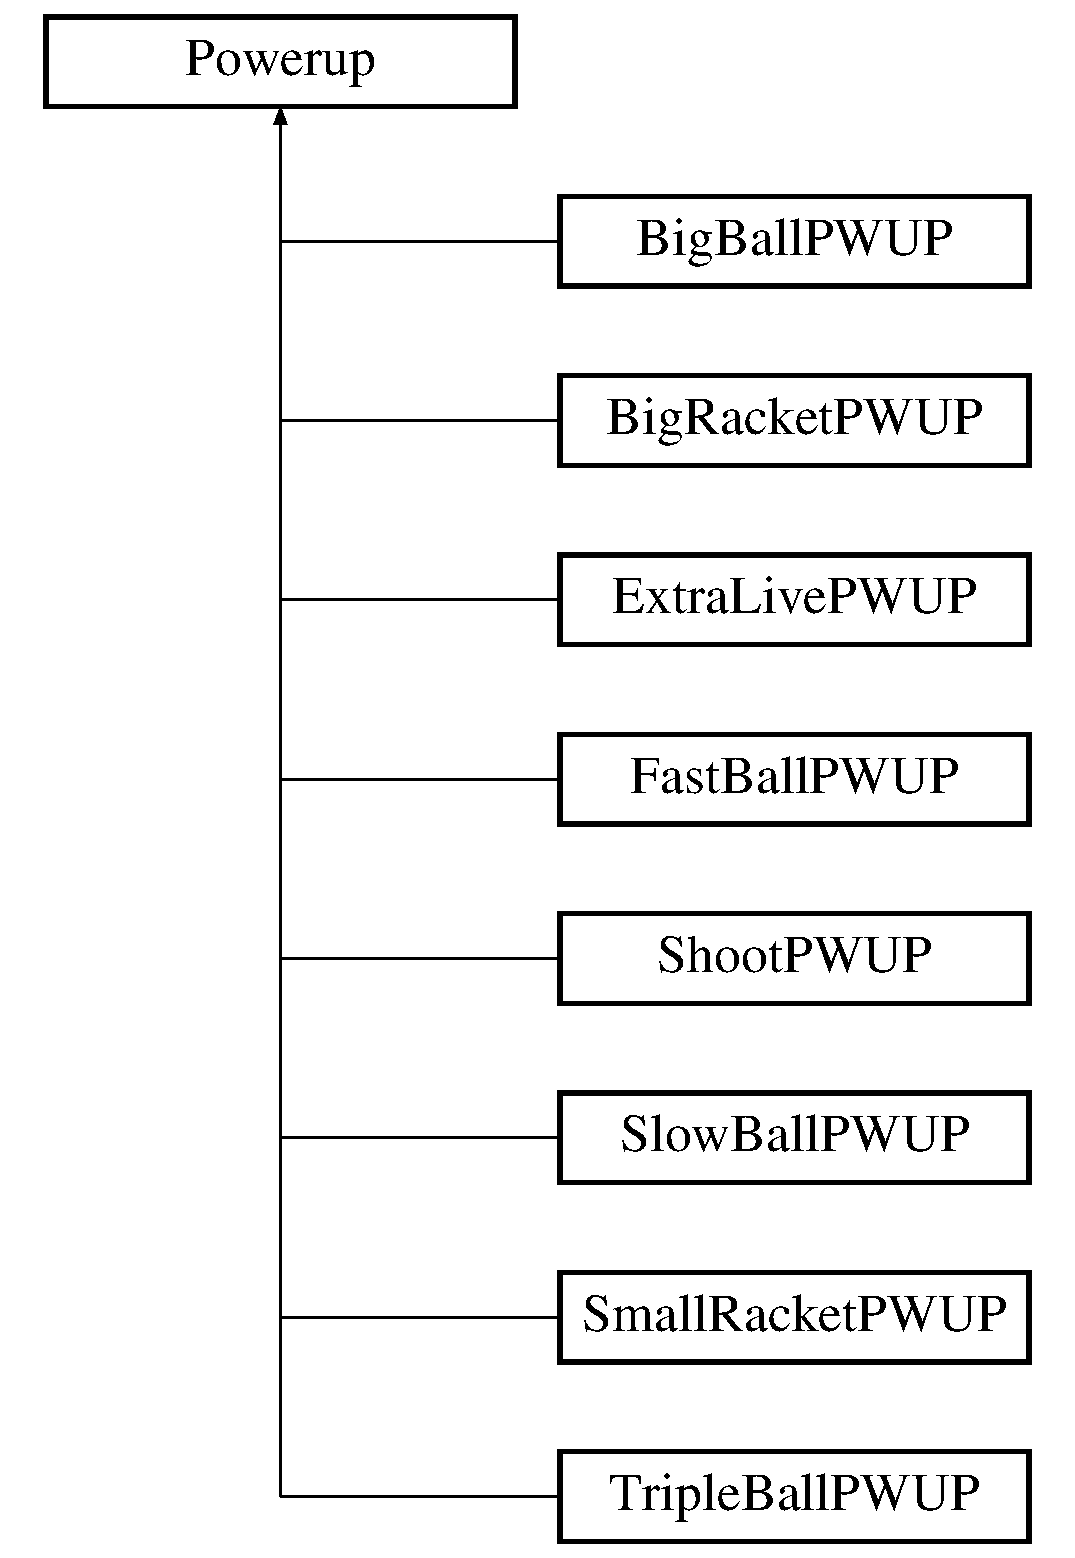
\includegraphics[height=9.000000cm]{class_powerup}
\end{center}
\end{figure}
\subsection*{Public Member Functions}
\begin{DoxyCompactItemize}
\item 
\mbox{\Hypertarget{class_powerup_ab4bdb1e3b63095c936d2505ffce31f3e}\label{class_powerup_ab4bdb1e3b63095c936d2505ffce31f3e}} 
{\bfseries Powerup} (double xx, double yy)
\item 
\mbox{\Hypertarget{class_powerup_a8a2434d845b29044736c2618b1fce1db}\label{class_powerup_a8a2434d845b29044736c2618b1fce1db}} 
void {\bfseries Destroy} ()
\item 
\mbox{\Hypertarget{class_powerup_a27c8857f4e41c6d09efcc4447a9102cf}\label{class_powerup_a27c8857f4e41c6d09efcc4447a9102cf}} 
virtual void \hyperlink{class_powerup_a27c8857f4e41c6d09efcc4447a9102cf}{Collect} ()
\begin{DoxyCompactList}\small\item\em Calls effect the powerup has on player when collected. \end{DoxyCompactList}\item 
char \hyperlink{class_powerup_a5e81fffa256f0f339c4ac430d897a1ae}{Move} (float time\+Step)
\begin{DoxyCompactList}\small\item\em Calculates new position, checks for collision. \end{DoxyCompactList}\end{DoxyCompactItemize}
\subsection*{Static Public Member Functions}
\begin{DoxyCompactItemize}
\item 
static void \hyperlink{class_powerup_a0a9b0365e47a25e5bee5112357d7d1cd}{Move\+All} (float time\+Step)
\begin{DoxyCompactList}\small\item\em Calls \hyperlink{class_powerup_a5e81fffa256f0f339c4ac430d897a1ae}{Move()} on all powerups in powerup\+List. \end{DoxyCompactList}\end{DoxyCompactItemize}
\subsection*{Public Attributes}
\begin{DoxyCompactItemize}
\item 
\mbox{\Hypertarget{class_powerup_ac021dce376ab3946c8bb9f13add88f9c}\label{class_powerup_ac021dce376ab3946c8bb9f13add88f9c}} 
double \hyperlink{class_powerup_ac021dce376ab3946c8bb9f13add88f9c}{x}
\begin{DoxyCompactList}\small\item\em X coordinate. \end{DoxyCompactList}\item 
\mbox{\Hypertarget{class_powerup_af28a919bbed400c8e213d69e25d6a864}\label{class_powerup_af28a919bbed400c8e213d69e25d6a864}} 
double \hyperlink{class_powerup_af28a919bbed400c8e213d69e25d6a864}{y}
\begin{DoxyCompactList}\small\item\em Y coordinate. \end{DoxyCompactList}\item 
\mbox{\Hypertarget{class_powerup_a219f4a4c1e6d9c0cb6ee60a03c3d9046}\label{class_powerup_a219f4a4c1e6d9c0cb6ee60a03c3d9046}} 
double \hyperlink{class_powerup_a219f4a4c1e6d9c0cb6ee60a03c3d9046}{Vy}
\begin{DoxyCompactList}\small\item\em Vertical speed of powerup. \end{DoxyCompactList}\item 
\mbox{\Hypertarget{class_powerup_a852c3a59988fe5067c5ebef799c50740}\label{class_powerup_a852c3a59988fe5067c5ebef799c50740}} 
\hyperlink{struct_colour}{Colour} \hyperlink{class_powerup_a852c3a59988fe5067c5ebef799c50740}{color}
\begin{DoxyCompactList}\small\item\em \hyperlink{struct_colour}{Colour} of powerup. \end{DoxyCompactList}\end{DoxyCompactItemize}


\subsection{Detailed Description}
Class for powerups. 

\subsection{Member Function Documentation}
\mbox{\Hypertarget{class_powerup_a5e81fffa256f0f339c4ac430d897a1ae}\label{class_powerup_a5e81fffa256f0f339c4ac430d897a1ae}} 
\index{Powerup@{Powerup}!Move@{Move}}
\index{Move@{Move}!Powerup@{Powerup}}
\subsubsection{\texorpdfstring{Move()}{Move()}}
{\footnotesize\ttfamily char Powerup\+::\+Move (\begin{DoxyParamCaption}\item[{float}]{time\+Step }\end{DoxyParamCaption})\hspace{0.3cm}{\ttfamily [inline]}}



Calculates new position, checks for collision. 


\begin{DoxyParams}{Parameters}
{\em float} & time\+Step.\\
\hline
\end{DoxyParams}
\begin{DoxyReturn}{Returns}
char -\/1 When out of boundaries. 

char 1 else 
\end{DoxyReturn}
\mbox{\Hypertarget{class_powerup_a0a9b0365e47a25e5bee5112357d7d1cd}\label{class_powerup_a0a9b0365e47a25e5bee5112357d7d1cd}} 
\index{Powerup@{Powerup}!Move\+All@{Move\+All}}
\index{Move\+All@{Move\+All}!Powerup@{Powerup}}
\subsubsection{\texorpdfstring{Move\+All()}{MoveAll()}}
{\footnotesize\ttfamily static void Powerup\+::\+Move\+All (\begin{DoxyParamCaption}\item[{float}]{time\+Step }\end{DoxyParamCaption})\hspace{0.3cm}{\ttfamily [inline]}, {\ttfamily [static]}}



Calls \hyperlink{class_powerup_a5e81fffa256f0f339c4ac430d897a1ae}{Move()} on all powerups in powerup\+List. 


\begin{DoxyParams}{Parameters}
{\em float} & time\+Step \\
\hline
\end{DoxyParams}


The documentation for this class was generated from the following file\+:\begin{DoxyCompactItemize}
\item 
Arkanoid/Powerup.\+h\end{DoxyCompactItemize}

\hypertarget{class_racket}{}\section{Racket Class Reference}
\label{class_racket}\index{Racket@{Racket}}


Class for racket.  




{\ttfamily \#include $<$Racket.\+h$>$}

\subsection*{Public Member Functions}
\begin{DoxyCompactItemize}
\item 
int \hyperlink{class_racket_aed265c7633d22165e3ad30b4dfa6c7f8}{Move} (float)
\begin{DoxyCompactList}\small\item\em Moves the racket, based on its speed. \end{DoxyCompactList}\end{DoxyCompactItemize}
\subsection*{Static Public Member Functions}
\begin{DoxyCompactItemize}
\item 
\mbox{\Hypertarget{class_racket_a4f0c0c96b24dedc89b29862ac9b47ccd}\label{class_racket_a4f0c0c96b24dedc89b29862ac9b47ccd}} 
static \hyperlink{class_racket}{Racket} \& {\bfseries get\+Instance} ()
\end{DoxyCompactItemize}
\subsection*{Public Attributes}
\begin{DoxyCompactItemize}
\item 
\mbox{\Hypertarget{class_racket_a983c4183fdc7338ddfc0bc1696cf93eb}\label{class_racket_a983c4183fdc7338ddfc0bc1696cf93eb}} 
double \hyperlink{class_racket_a983c4183fdc7338ddfc0bc1696cf93eb}{speed}
\begin{DoxyCompactList}\small\item\em Speed of the racket. \end{DoxyCompactList}\item 
\mbox{\Hypertarget{class_racket_a13391bbcabb61d9df5558865971e43f8}\label{class_racket_a13391bbcabb61d9df5558865971e43f8}} 
double \hyperlink{class_racket_a13391bbcabb61d9df5558865971e43f8}{width}
\begin{DoxyCompactList}\small\item\em Width of the racket, from center. \end{DoxyCompactList}\item 
\mbox{\Hypertarget{class_racket_abbee058cfc982a0726e81ee7d9e6a34e}\label{class_racket_abbee058cfc982a0726e81ee7d9e6a34e}} 
double \hyperlink{class_racket_abbee058cfc982a0726e81ee7d9e6a34e}{x}
\begin{DoxyCompactList}\small\item\em X coordinate. Center of racket. \end{DoxyCompactList}\item 
\mbox{\Hypertarget{class_racket_abc335dd83b72c2008f32c1130aac70d4}\label{class_racket_abc335dd83b72c2008f32c1130aac70d4}} 
double \hyperlink{class_racket_abc335dd83b72c2008f32c1130aac70d4}{y}
\begin{DoxyCompactList}\small\item\em Y coordinate. \end{DoxyCompactList}\item 
\mbox{\Hypertarget{class_racket_a080094786cc70722b80f34bcf88b7694}\label{class_racket_a080094786cc70722b80f34bcf88b7694}} 
char \hyperlink{class_racket_a080094786cc70722b80f34bcf88b7694}{shooting\+Enabled}
\begin{DoxyCompactList}\small\item\em Defining if shooting is possible. \end{DoxyCompactList}\end{DoxyCompactItemize}


\subsection{Detailed Description}
Class for racket. 

\subsection{Member Function Documentation}
\mbox{\Hypertarget{class_racket_aed265c7633d22165e3ad30b4dfa6c7f8}\label{class_racket_aed265c7633d22165e3ad30b4dfa6c7f8}} 
\index{Racket@{Racket}!Move@{Move}}
\index{Move@{Move}!Racket@{Racket}}
\subsubsection{\texorpdfstring{Move()}{Move()}}
{\footnotesize\ttfamily int Racket\+::\+Move (\begin{DoxyParamCaption}\item[{float}]{time\+Step }\end{DoxyParamCaption})}



Moves the racket, based on its speed. 


\begin{DoxyParams}{Parameters}
{\em float} & time\+Step\\
\hline
\end{DoxyParams}
\begin{DoxyReturn}{Returns}
0 If border is hit. 
\end{DoxyReturn}


The documentation for this class was generated from the following files\+:\begin{DoxyCompactItemize}
\item 
Arkanoid/Racket.\+h\item 
Arkanoid/Racket.\+cpp\end{DoxyCompactItemize}

\hypertarget{class_regular_block}{}\section{Regular\+Block Class Reference}
\label{class_regular_block}\index{Regular\+Block@{Regular\+Block}}


Regular block with health = R\+E\+G\+U\+L\+A\+R\+\_\+\+B\+L\+O\+C\+K\+\_\+\+H\+E\+A\+L\+TH (\hyperlink{_config_8h_source}{config.\+h})  




{\ttfamily \#include $<$Block.\+h$>$}

Inheritance diagram for Regular\+Block\+:\begin{figure}[H]
\begin{center}
\leavevmode
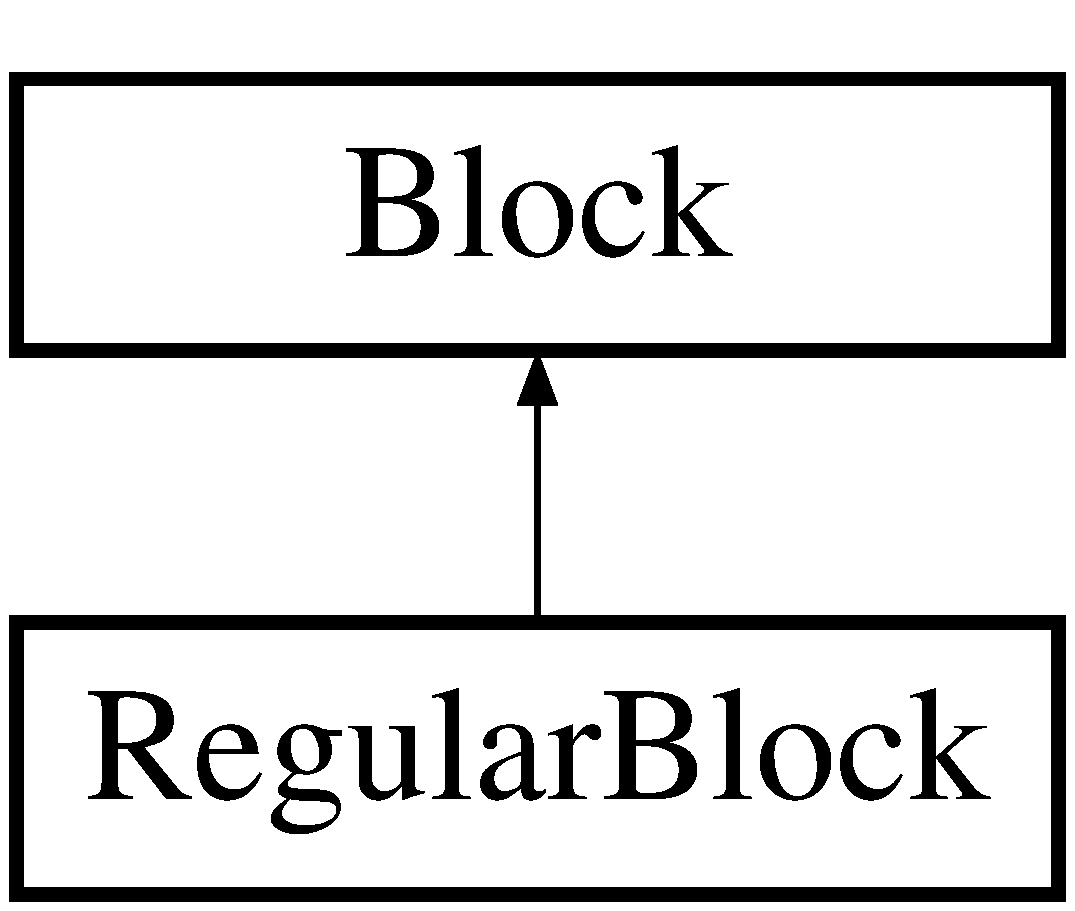
\includegraphics[height=2.000000cm]{class_regular_block}
\end{center}
\end{figure}
\subsection*{Public Member Functions}
\begin{DoxyCompactItemize}
\item 
\mbox{\Hypertarget{class_regular_block_ae9eba20f97d945197d7ce511fd64daa6}\label{class_regular_block_ae9eba20f97d945197d7ce511fd64daa6}} 
{\bfseries Regular\+Block} (char hlt=R\+E\+G\+U\+L\+A\+R\+\_\+\+B\+L\+O\+C\+K\+\_\+\+H\+E\+A\+L\+TH, unsigned char r=0, unsigned char g=255, unsigned char b=0, unsigned char a=255)
\end{DoxyCompactItemize}
\subsection*{Additional Inherited Members}


\subsection{Detailed Description}
Regular block with health = R\+E\+G\+U\+L\+A\+R\+\_\+\+B\+L\+O\+C\+K\+\_\+\+H\+E\+A\+L\+TH (\hyperlink{_config_8h_source}{config.\+h}) 

The documentation for this class was generated from the following file\+:\begin{DoxyCompactItemize}
\item 
Arkanoid/Block.\+h\end{DoxyCompactItemize}

\hypertarget{class_render}{}\section{Render Class Reference}
\label{class_render}\index{Render@{Render}}


Class containing some methods and texture pointers for rendering.  




{\ttfamily \#include $<$Render.\+h$>$}

\subsection*{Static Public Member Functions}
\begin{DoxyCompactItemize}
\item 
\mbox{\Hypertarget{class_render_adec8165d47785008ef1b593cd7f2866f}\label{class_render_adec8165d47785008ef1b593cd7f2866f}} 
static \hyperlink{class_render}{Render} \& {\bfseries get\+Instance} ()
\item 
\mbox{\Hypertarget{class_render_aa0e41ce94983c5ead71a3a2bff83b62b}\label{class_render_aa0e41ce94983c5ead71a3a2bff83b62b}} 
static void {\bfseries Render\+Balls} ()
\item 
\mbox{\Hypertarget{class_render_ab14b3c69b68bb08457d9416426a291f2}\label{class_render_ab14b3c69b68bb08457d9416426a291f2}} 
static void {\bfseries Render\+Blocks} ()
\item 
\mbox{\Hypertarget{class_render_a4a257b71e0f6de8639e00c61a560662d}\label{class_render_a4a257b71e0f6de8639e00c61a560662d}} 
static void {\bfseries Render\+Racket} ()
\item 
\mbox{\Hypertarget{class_render_a2d2dbb588a127236e25106d63e2e031d}\label{class_render_a2d2dbb588a127236e25106d63e2e031d}} 
static void {\bfseries Render\+Pwups} ()
\item 
\mbox{\Hypertarget{class_render_af79f3fef9fceb2615207f5b9feecf014}\label{class_render_af79f3fef9fceb2615207f5b9feecf014}} 
static void {\bfseries Render\+Bullets} ()
\item 
\mbox{\Hypertarget{class_render_af07aacd067217ff6ee66067a374e9397}\label{class_render_af07aacd067217ff6ee66067a374e9397}} 
static void {\bfseries Render\+Enemies} ()
\end{DoxyCompactItemize}
\subsection*{Public Attributes}
\begin{DoxyCompactItemize}
\item 
\mbox{\Hypertarget{class_render_a56f4679c30a4da025f82f93847d8489a}\label{class_render_a56f4679c30a4da025f82f93847d8489a}} 
S\+D\+L\+\_\+\+Window $\ast$ {\bfseries g\+Window} = N\+U\+LL
\item 
\mbox{\Hypertarget{class_render_afa0976cec27200747482493e6e9ca779}\label{class_render_afa0976cec27200747482493e6e9ca779}} 
S\+D\+L\+\_\+\+Renderer $\ast$ {\bfseries g\+Renderer} = N\+U\+LL
\item 
\mbox{\Hypertarget{class_render_af698eaede8e7778ca77187baaaeb8cbe}\label{class_render_af698eaede8e7778ca77187baaaeb8cbe}} 
S\+D\+L\+\_\+\+Rect {\bfseries left\+Viewport} = \{ 0, 0, S\+C\+R\+E\+E\+N\+\_\+\+W\+I\+D\+TH, S\+C\+R\+E\+E\+N\+\_\+\+H\+E\+I\+G\+HT \}
\item 
\mbox{\Hypertarget{class_render_af4e82c87974121b37bbbcb001cc46a83}\label{class_render_af4e82c87974121b37bbbcb001cc46a83}} 
S\+D\+L\+\_\+\+Rect {\bfseries right\+Viewport} = \{ S\+C\+R\+E\+E\+N\+\_\+\+W\+I\+D\+TH + 1, 0, S\+C\+R\+E\+E\+N\+\_\+\+W\+I\+D\+TH + S\+I\+D\+E\+B\+A\+R\+\_\+\+W\+I\+D\+TH, S\+C\+R\+E\+E\+N\+\_\+\+H\+E\+I\+G\+HT \}
\item 
\mbox{\Hypertarget{class_render_a5c144f87e4aa2ef8643a8e2dc139e478}\label{class_render_a5c144f87e4aa2ef8643a8e2dc139e478}} 
\hyperlink{class_l_texture}{L\+Texture} \hyperlink{class_render_a5c144f87e4aa2ef8643a8e2dc139e478}{g\+Ball\+Texture}
\begin{DoxyCompactList}\small\item\em Scene textures. \end{DoxyCompactList}\item 
\mbox{\Hypertarget{class_render_aca8afc8957a810bb962ab8f5a31d8500}\label{class_render_aca8afc8957a810bb962ab8f5a31d8500}} 
\hyperlink{class_l_texture}{L\+Texture} {\bfseries g\+Block\+Texture}
\item 
\mbox{\Hypertarget{class_render_a948ab1b6efa9c18ec8fde021cd745963}\label{class_render_a948ab1b6efa9c18ec8fde021cd745963}} 
\hyperlink{class_l_texture}{L\+Texture} {\bfseries g\+Racket\+Texture}
\item 
\mbox{\Hypertarget{class_render_a0c4f77794b5dabecf25f84415fb3ad85}\label{class_render_a0c4f77794b5dabecf25f84415fb3ad85}} 
\hyperlink{class_l_texture}{L\+Texture} {\bfseries g\+Racket\+Texture2}
\item 
\mbox{\Hypertarget{class_render_a02ca1847aad2235c4c703f4f4ee20b78}\label{class_render_a02ca1847aad2235c4c703f4f4ee20b78}} 
\hyperlink{class_l_texture}{L\+Texture} {\bfseries g\+Pwup\+Texture}
\item 
\mbox{\Hypertarget{class_render_a8c281707bee4ff9460abf48e2fbf0f9c}\label{class_render_a8c281707bee4ff9460abf48e2fbf0f9c}} 
\hyperlink{class_l_texture}{L\+Texture} {\bfseries g\+Bullet\+Texture}
\item 
\mbox{\Hypertarget{class_render_a34a83802700f31426f018fb201d412dc}\label{class_render_a34a83802700f31426f018fb201d412dc}} 
\hyperlink{class_l_texture}{L\+Texture} {\bfseries g\+Text\+Texture}
\item 
\mbox{\Hypertarget{class_render_af3847d2c17f0062661e6b8c0b06170db}\label{class_render_af3847d2c17f0062661e6b8c0b06170db}} 
\hyperlink{class_l_texture}{L\+Texture} {\bfseries g\+Enemy\+Texture}
\item 
\mbox{\Hypertarget{class_render_af372a476ddfb76f9e641ca629766daff}\label{class_render_af372a476ddfb76f9e641ca629766daff}} 
T\+T\+F\+\_\+\+Font $\ast$ {\bfseries g\+Font} = 0
\item 
\mbox{\Hypertarget{class_render_af2b513498a39277236db315092995f5b}\label{class_render_af2b513498a39277236db315092995f5b}} 
Mix\+\_\+\+Chunk $\ast$ {\bfseries g\+Ping} = N\+U\+LL
\item 
\mbox{\Hypertarget{class_render_a018ac074d1596fdc0f5cc6f474605ec9}\label{class_render_a018ac074d1596fdc0f5cc6f474605ec9}} 
Mix\+\_\+\+Chunk $\ast$ {\bfseries g\+Racket\+Pong} = N\+U\+LL
\end{DoxyCompactItemize}


\subsection{Detailed Description}
Class containing some methods and texture pointers for rendering. 

The documentation for this class was generated from the following files\+:\begin{DoxyCompactItemize}
\item 
Arkanoid/Render.\+h\item 
Arkanoid/Render.\+cpp\end{DoxyCompactItemize}

\hypertarget{struct_save_data}{}\section{Save\+Data Struct Reference}
\label{struct_save_data}\index{Save\+Data@{Save\+Data}}


A temporary struct to easen saving/loading procedure.  




{\ttfamily \#include $<$Player.\+h$>$}

\subsection*{Public Member Functions}
\begin{DoxyCompactItemize}
\item 
\mbox{\Hypertarget{struct_save_data_aadbe80f0e50ca006c4ab551e354dffd4}\label{struct_save_data_aadbe80f0e50ca006c4ab551e354dffd4}} 
void {\bfseries Load\+From\+Player} ()
\end{DoxyCompactItemize}
\subsection*{Public Attributes}
\begin{DoxyCompactItemize}
\item 
\mbox{\Hypertarget{struct_save_data_a97845f98c55e065474a64da106613c64}\label{struct_save_data_a97845f98c55e065474a64da106613c64}} 
int {\bfseries level}
\item 
\mbox{\Hypertarget{struct_save_data_af45bd67901ef6353a5d18853cf12afca}\label{struct_save_data_af45bd67901ef6353a5d18853cf12afca}} 
int {\bfseries score}
\item 
\mbox{\Hypertarget{struct_save_data_a3c77e3bbee8113a1ace50ee6bf5e6563}\label{struct_save_data_a3c77e3bbee8113a1ace50ee6bf5e6563}} 
int {\bfseries lives}
\item 
\mbox{\Hypertarget{struct_save_data_a54238e0683a22713a69a5bc1bd3cebd6}\label{struct_save_data_a54238e0683a22713a69a5bc1bd3cebd6}} 
int {\bfseries difficulty}
\end{DoxyCompactItemize}
\subsection*{Friends}
\begin{DoxyCompactItemize}
\item 
\mbox{\Hypertarget{struct_save_data_a1bb052bd966adbcac481f7465303bf01}\label{struct_save_data_a1bb052bd966adbcac481f7465303bf01}} 
std\+::ostream \& {\bfseries operator$<$$<$} (std\+::ostream \&os, const \hyperlink{struct_save_data}{Save\+Data} \&obj)
\item 
\mbox{\Hypertarget{struct_save_data_a734fceef19cc9a9c220a1989368fb176}\label{struct_save_data_a734fceef19cc9a9c220a1989368fb176}} 
std\+::istream \& {\bfseries operator$>$$>$} (std\+::istream \&is, \hyperlink{struct_save_data}{Save\+Data} \&obj)
\end{DoxyCompactItemize}


\subsection{Detailed Description}
A temporary struct to easen saving/loading procedure. 

The documentation for this struct was generated from the following file\+:\begin{DoxyCompactItemize}
\item 
Arkanoid/Player.\+h\end{DoxyCompactItemize}

\hypertarget{class_shoot_p_w_u_p}{}\section{Shoot\+P\+W\+UP Class Reference}
\label{class_shoot_p_w_u_p}\index{Shoot\+P\+W\+UP@{Shoot\+P\+W\+UP}}


\hyperlink{class_powerup}{Powerup} that gives ability to shoot missiles.  




{\ttfamily \#include $<$Powerup.\+h$>$}

Inheritance diagram for Shoot\+P\+W\+UP\+:\begin{figure}[H]
\begin{center}
\leavevmode
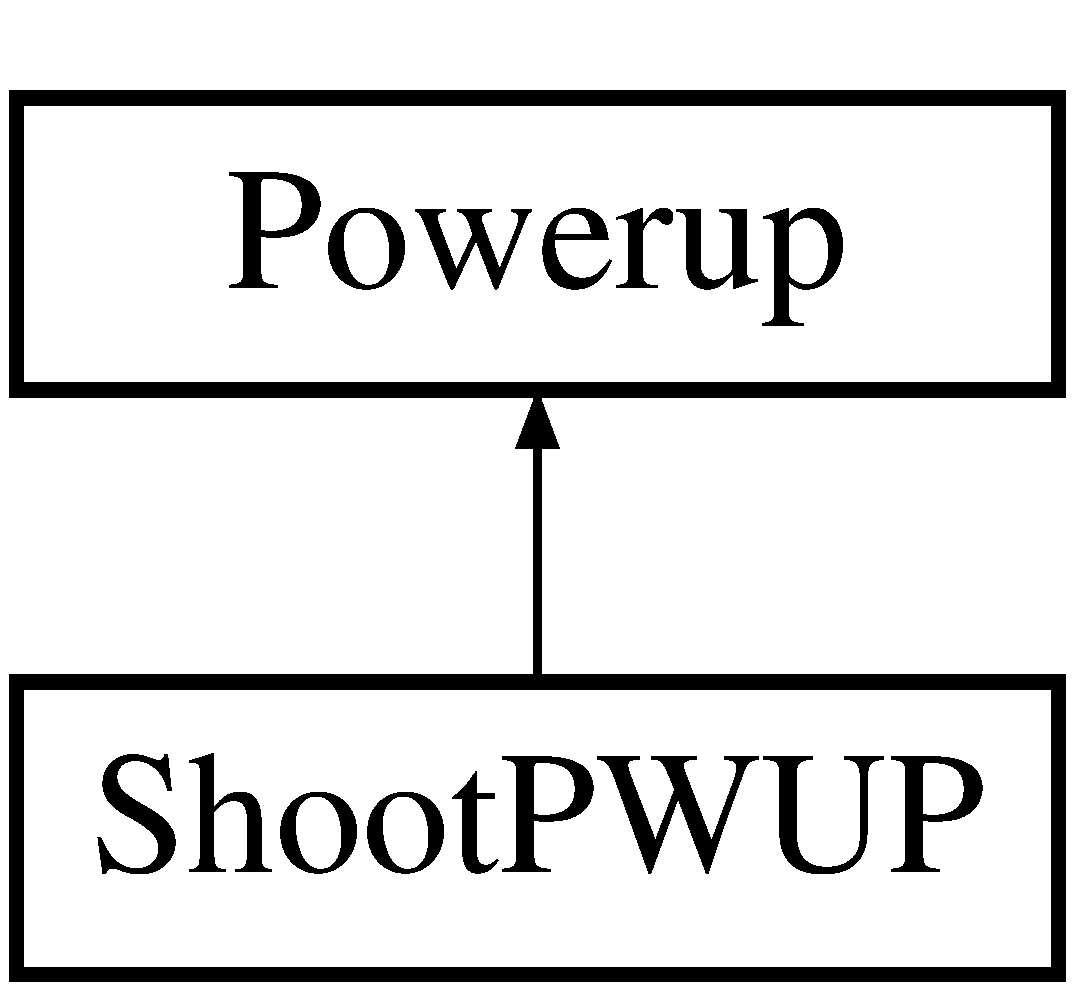
\includegraphics[height=2.000000cm]{class_shoot_p_w_u_p}
\end{center}
\end{figure}
\subsection*{Public Member Functions}
\begin{DoxyCompactItemize}
\item 
\mbox{\Hypertarget{class_shoot_p_w_u_p_a20a366283557399867950a55c5c2140b}\label{class_shoot_p_w_u_p_a20a366283557399867950a55c5c2140b}} 
void \hyperlink{class_shoot_p_w_u_p_a20a366283557399867950a55c5c2140b}{Collect} ()
\begin{DoxyCompactList}\small\item\em Calls effect the powerup has on player when collected. \end{DoxyCompactList}\item 
\mbox{\Hypertarget{class_shoot_p_w_u_p_ac38d8f9467b29a21ef89fe8eb24f80d1}\label{class_shoot_p_w_u_p_ac38d8f9467b29a21ef89fe8eb24f80d1}} 
{\bfseries Shoot\+P\+W\+UP} (double xx, double yy)
\end{DoxyCompactItemize}
\subsection*{Additional Inherited Members}


\subsection{Detailed Description}
\hyperlink{class_powerup}{Powerup} that gives ability to shoot missiles. 

The documentation for this class was generated from the following file\+:\begin{DoxyCompactItemize}
\item 
Arkanoid/Powerup.\+h\end{DoxyCompactItemize}

\hypertarget{class_slow_ball_p_w_u_p}{}\section{Slow\+Ball\+P\+W\+UP Class Reference}
\label{class_slow_ball_p_w_u_p}\index{Slow\+Ball\+P\+W\+UP@{Slow\+Ball\+P\+W\+UP}}


\hyperlink{class_powerup}{Powerup} decrasing the speed of balls.  




{\ttfamily \#include $<$Powerup.\+h$>$}

Inheritance diagram for Slow\+Ball\+P\+W\+UP\+:\begin{figure}[H]
\begin{center}
\leavevmode
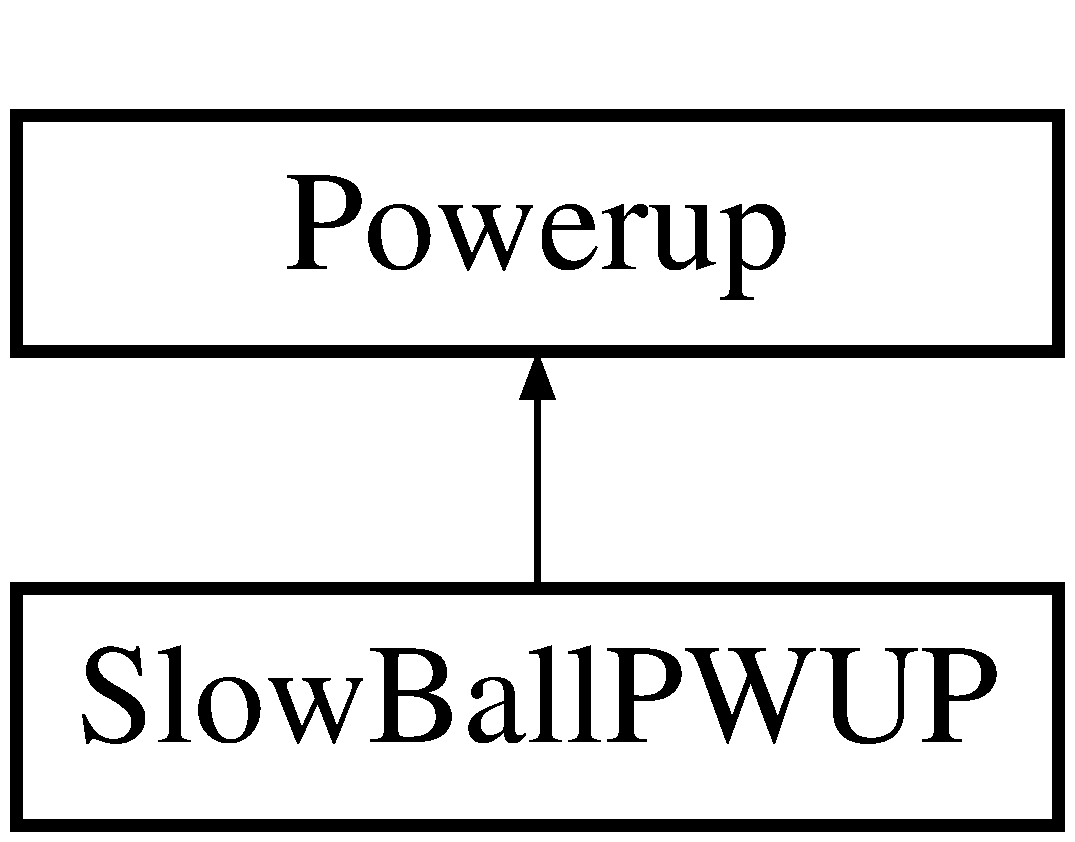
\includegraphics[height=2.000000cm]{class_slow_ball_p_w_u_p}
\end{center}
\end{figure}
\subsection*{Public Member Functions}
\begin{DoxyCompactItemize}
\item 
\mbox{\Hypertarget{class_slow_ball_p_w_u_p_ad1cd4576b80a5e33abb11e77482cf9c8}\label{class_slow_ball_p_w_u_p_ad1cd4576b80a5e33abb11e77482cf9c8}} 
void \hyperlink{class_slow_ball_p_w_u_p_ad1cd4576b80a5e33abb11e77482cf9c8}{Collect} ()
\begin{DoxyCompactList}\small\item\em Calls effect the powerup has on player when collected. \end{DoxyCompactList}\item 
\mbox{\Hypertarget{class_slow_ball_p_w_u_p_ad4454483d00e04e90b54f5439b64e0b1}\label{class_slow_ball_p_w_u_p_ad4454483d00e04e90b54f5439b64e0b1}} 
{\bfseries Slow\+Ball\+P\+W\+UP} (double xx, double yy)
\end{DoxyCompactItemize}
\subsection*{Additional Inherited Members}


\subsection{Detailed Description}
\hyperlink{class_powerup}{Powerup} decrasing the speed of balls. 

The documentation for this class was generated from the following file\+:\begin{DoxyCompactItemize}
\item 
Arkanoid/Powerup.\+h\end{DoxyCompactItemize}

\hypertarget{class_small_racket_p_w_u_p}{}\section{Small\+Racket\+P\+W\+UP Class Reference}
\label{class_small_racket_p_w_u_p}\index{Small\+Racket\+P\+W\+UP@{Small\+Racket\+P\+W\+UP}}


\hyperlink{class_powerup}{Powerup} decrasing the size of \hyperlink{class_racket}{Racket}.  




{\ttfamily \#include $<$Powerup.\+h$>$}

Inheritance diagram for Small\+Racket\+P\+W\+UP\+:\begin{figure}[H]
\begin{center}
\leavevmode
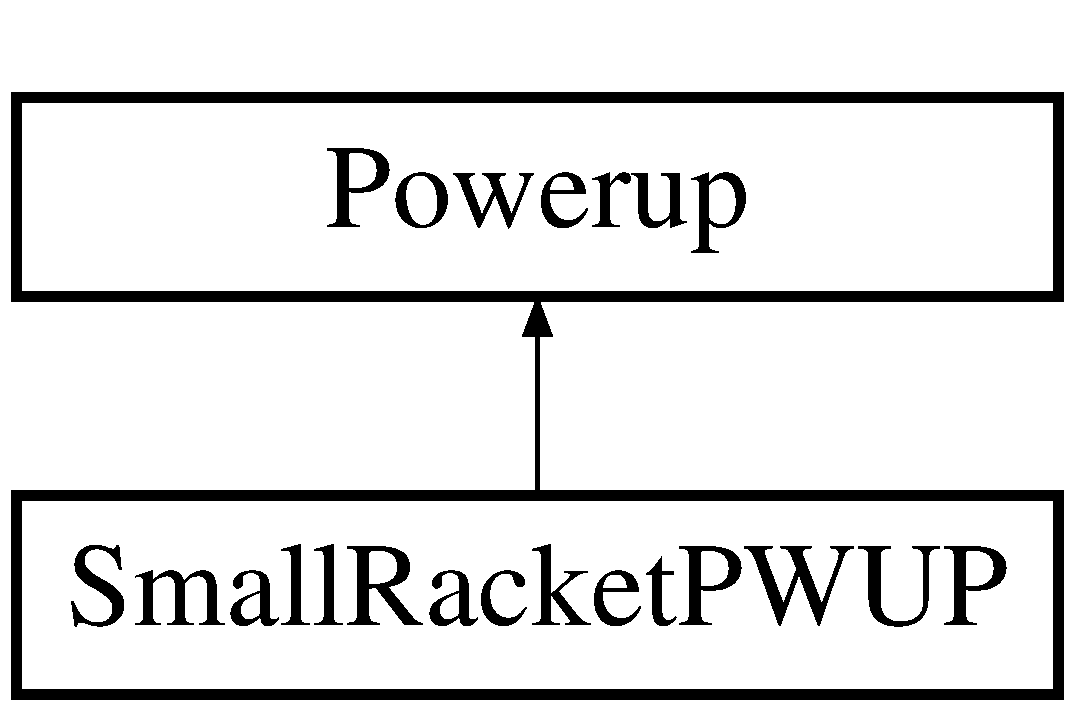
\includegraphics[height=2.000000cm]{class_small_racket_p_w_u_p}
\end{center}
\end{figure}
\subsection*{Public Member Functions}
\begin{DoxyCompactItemize}
\item 
\mbox{\Hypertarget{class_small_racket_p_w_u_p_a59ce615ac639d1f30361ad1bf2d4c496}\label{class_small_racket_p_w_u_p_a59ce615ac639d1f30361ad1bf2d4c496}} 
void \hyperlink{class_small_racket_p_w_u_p_a59ce615ac639d1f30361ad1bf2d4c496}{Collect} ()
\begin{DoxyCompactList}\small\item\em Calls effect the powerup has on player when collected. \end{DoxyCompactList}\item 
\mbox{\Hypertarget{class_small_racket_p_w_u_p_ac7739eb07b5e83df20ffba1ae0aa7129}\label{class_small_racket_p_w_u_p_ac7739eb07b5e83df20ffba1ae0aa7129}} 
{\bfseries Small\+Racket\+P\+W\+UP} (double xx, double yy)
\end{DoxyCompactItemize}
\subsection*{Additional Inherited Members}


\subsection{Detailed Description}
\hyperlink{class_powerup}{Powerup} decrasing the size of \hyperlink{class_racket}{Racket}. 

The documentation for this class was generated from the following file\+:\begin{DoxyCompactItemize}
\item 
Arkanoid/Powerup.\+h\end{DoxyCompactItemize}

\hypertarget{class_strong_block}{}\section{Strong\+Block Class Reference}
\label{class_strong_block}\index{Strong\+Block@{Strong\+Block}}


Stronger block with health = S\+T\+R\+O\+N\+G\+\_\+\+B\+L\+O\+C\+K\+\_\+\+H\+E\+A\+L\+TH (\hyperlink{_config_8h_source}{config.\+h})  




{\ttfamily \#include $<$Block.\+h$>$}

Inheritance diagram for Strong\+Block\+:\begin{figure}[H]
\begin{center}
\leavevmode
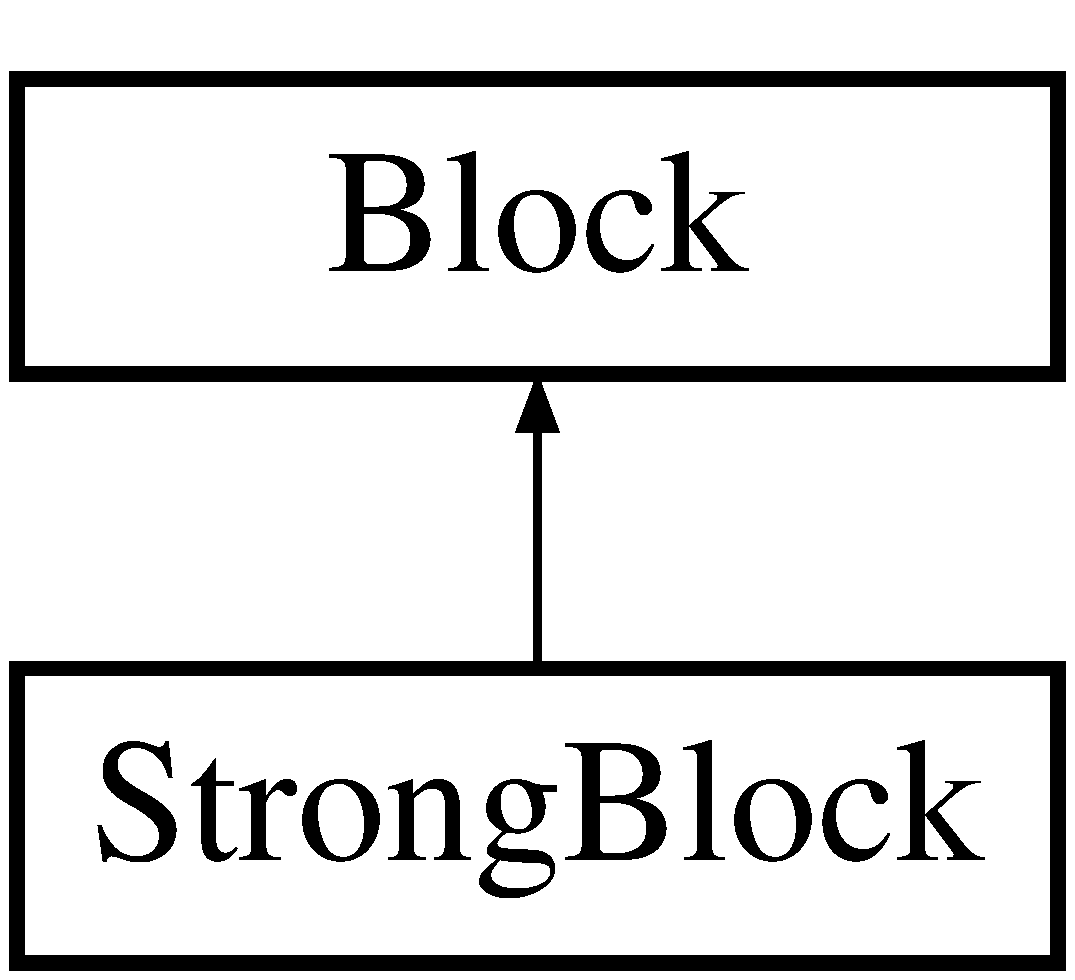
\includegraphics[height=2.000000cm]{class_strong_block}
\end{center}
\end{figure}
\subsection*{Public Member Functions}
\begin{DoxyCompactItemize}
\item 
\mbox{\Hypertarget{class_strong_block_aeb0de776e3a9bb226f922e9f92832338}\label{class_strong_block_aeb0de776e3a9bb226f922e9f92832338}} 
{\bfseries Strong\+Block} (char hlt=S\+T\+R\+O\+N\+G\+\_\+\+B\+L\+O\+C\+K\+\_\+\+H\+E\+A\+L\+TH, unsigned char r=0, unsigned char g=0, unsigned char b=255, unsigned char a=255)
\end{DoxyCompactItemize}
\subsection*{Additional Inherited Members}


\subsection{Detailed Description}
Stronger block with health = S\+T\+R\+O\+N\+G\+\_\+\+B\+L\+O\+C\+K\+\_\+\+H\+E\+A\+L\+TH (\hyperlink{_config_8h_source}{config.\+h}) 

The documentation for this class was generated from the following file\+:\begin{DoxyCompactItemize}
\item 
Arkanoid/Block.\+h\end{DoxyCompactItemize}

\hypertarget{class_triple_ball_p_w_u_p}{}\section{Triple\+Ball\+P\+W\+UP Class Reference}
\label{class_triple_ball_p_w_u_p}\index{Triple\+Ball\+P\+W\+UP@{Triple\+Ball\+P\+W\+UP}}


\hyperlink{class_powerup}{Powerup} incrasing the amount of balls.  




{\ttfamily \#include $<$Powerup.\+h$>$}

Inheritance diagram for Triple\+Ball\+P\+W\+UP\+:\begin{figure}[H]
\begin{center}
\leavevmode
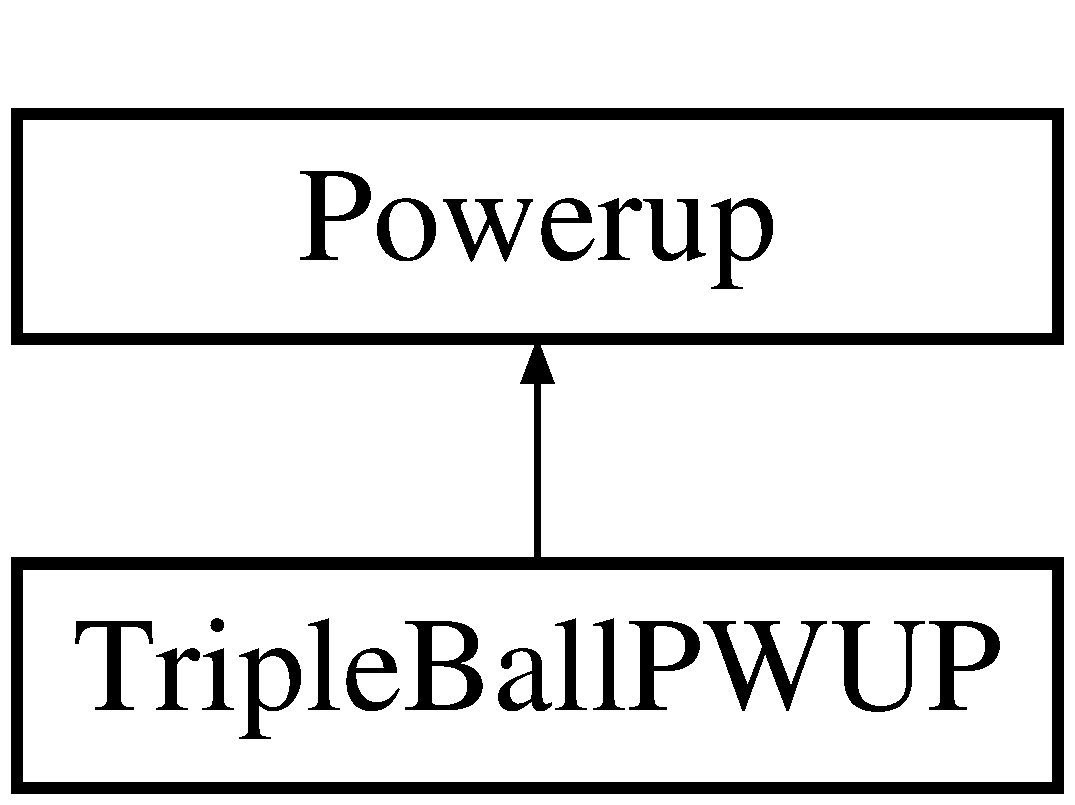
\includegraphics[height=2.000000cm]{class_triple_ball_p_w_u_p}
\end{center}
\end{figure}
\subsection*{Public Member Functions}
\begin{DoxyCompactItemize}
\item 
\mbox{\Hypertarget{class_triple_ball_p_w_u_p_ab4b1284f2edbe00bc9159fedb548032b}\label{class_triple_ball_p_w_u_p_ab4b1284f2edbe00bc9159fedb548032b}} 
void \hyperlink{class_triple_ball_p_w_u_p_ab4b1284f2edbe00bc9159fedb548032b}{Collect} ()
\begin{DoxyCompactList}\small\item\em Calls effect the powerup has on player when collected. \end{DoxyCompactList}\item 
\mbox{\Hypertarget{class_triple_ball_p_w_u_p_a1d139789a8b46027955699e69afbeb6f}\label{class_triple_ball_p_w_u_p_a1d139789a8b46027955699e69afbeb6f}} 
{\bfseries Triple\+Ball\+P\+W\+UP} (double xx, double yy)
\end{DoxyCompactItemize}
\subsection*{Additional Inherited Members}


\subsection{Detailed Description}
\hyperlink{class_powerup}{Powerup} incrasing the amount of balls. 

The documentation for this class was generated from the following file\+:\begin{DoxyCompactItemize}
\item 
Arkanoid/Powerup.\+h\end{DoxyCompactItemize}

\hypertarget{class_very_strong_block}{}\section{Very\+Strong\+Block Class Reference}
\label{class_very_strong_block}\index{Very\+Strong\+Block@{Very\+Strong\+Block}}


Even stronger block with health = V\+E\+R\+Y\+\_\+\+S\+T\+R\+O\+N\+G\+\_\+\+B\+L\+O\+C\+K\+\_\+\+H\+E\+A\+L\+TH (\hyperlink{_config_8h_source}{config.\+h})  




{\ttfamily \#include $<$Block.\+h$>$}

Inheritance diagram for Very\+Strong\+Block\+:\begin{figure}[H]
\begin{center}
\leavevmode
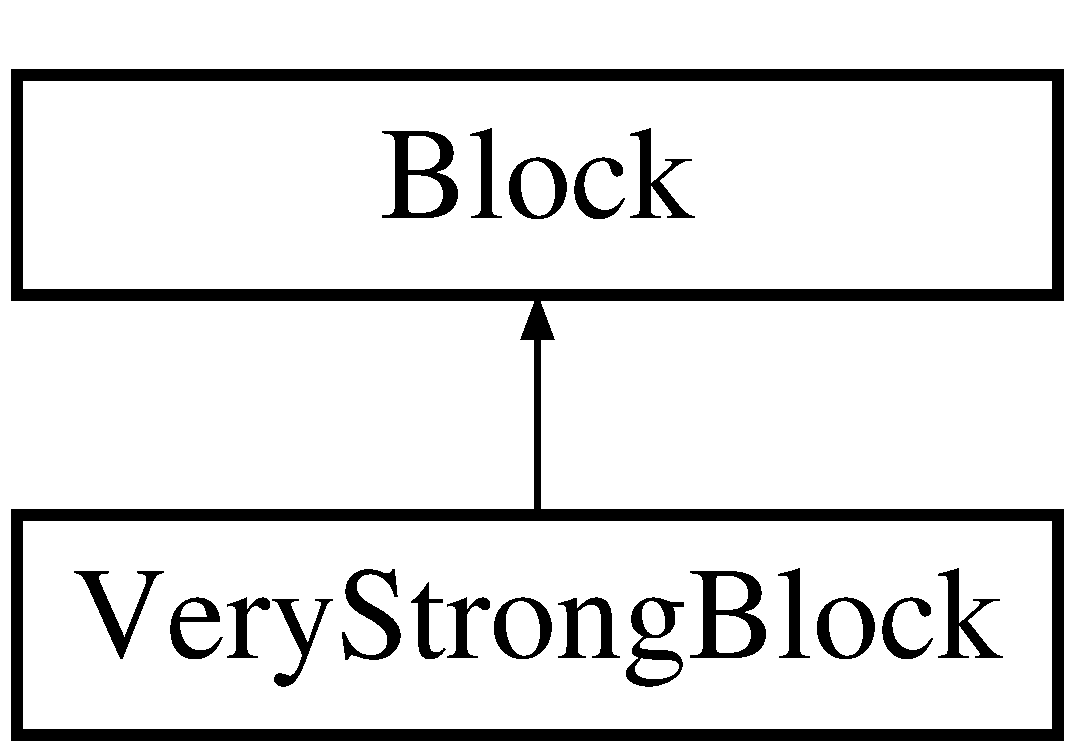
\includegraphics[height=2.000000cm]{class_very_strong_block}
\end{center}
\end{figure}
\subsection*{Public Member Functions}
\begin{DoxyCompactItemize}
\item 
\mbox{\Hypertarget{class_very_strong_block_a0566c718401694910412ef5b101d638e}\label{class_very_strong_block_a0566c718401694910412ef5b101d638e}} 
{\bfseries Very\+Strong\+Block} (char hlt=V\+E\+R\+Y\+\_\+\+S\+T\+R\+O\+N\+G\+\_\+\+B\+L\+O\+C\+K\+\_\+\+H\+E\+A\+L\+TH, unsigned char r=255, unsigned char g=255, unsigned char b=0, unsigned char a=255)
\end{DoxyCompactItemize}
\subsection*{Additional Inherited Members}


\subsection{Detailed Description}
Even stronger block with health = V\+E\+R\+Y\+\_\+\+S\+T\+R\+O\+N\+G\+\_\+\+B\+L\+O\+C\+K\+\_\+\+H\+E\+A\+L\+TH (\hyperlink{_config_8h_source}{config.\+h}) 

The documentation for this class was generated from the following file\+:\begin{DoxyCompactItemize}
\item 
Arkanoid/Block.\+h\end{DoxyCompactItemize}

%--- End generated contents ---

% Index
\backmatter
\newpage
\phantomsection
\clearemptydoublepage
\addcontentsline{toc}{chapter}{Index}
\printindex

\end{document}
